% !TEX root = main.tex
\documentclass[12pt,a4paper,oneside]{report}

% !TEX root = main.tex
\usepackage{fontspec}

% --- Times New Roman Font Setup ---
\setmainfont{TimesNewRoman-Regular.ttf}[
    Path = /home/ubuntu/ai-agent-crag/fonts/,
    BoldFont = TimesNewRoman-Bold.ttf,
    ItalicFont = TimesNewRoman-Italic.ttf,
    BoldItalicFont = TimesNewRoman-BoldItalic.ttf
]
\setmonofont{RobotoMono-Regular.ttf}[
    Path = /home/ubuntu/ai-agent-crag/fonts/,
    BoldFont = RobotoMono-Bold.ttf
]

\usepackage[a4paper, left=2.5cm, right=2.0cm, top=2.5cm, bottom=2.5cm]{geometry}
\usepackage[table]{xcolor}
\usepackage{graphicx}
\usepackage{booktabs}
\usepackage{tabularx}
\usepackage{colortbl}
\usepackage{array}
\usepackage{enumitem}
\usepackage{fancyhdr}
\usepackage{lastpage}
\usepackage{titlesec}
\usepackage{amsmath,amssymb}
\usepackage{listings}
\usepackage[most]{tcolorbox}
\usepackage{microtype}
\usepackage{caption}
\usepackage{setspace}
\usepackage[hidelinks, unicode, pdfencoding=auto]{hyperref}

% --- Line Spacing (Academic Standard: 1.25) ---
\setstretch{1.2}

% --- Color Palette (Neutral Academic Black & Grayscale) ---
\definecolor{primary}{HTML}{000000}      % Pure Black for titles & text
\definecolor{secondary}{HTML}{1A1A1A}    % Near Black
\definecolor{darkcharcoal}{HTML}{262626} % Neutral Dark
\definecolor{lightbg}{HTML}{F9FAFB}      % Soft background
\definecolor{bordergray}{HTML}{D1D5DB}   % Subtle borders
\definecolor{calloutbg}{HTML}{F8FAFC}    % Light neutral callout
\definecolor{calloutborder}{HTML}{4B5563}% Neutral slate border
\definecolor{callouttext}{HTML}{111827}  % Dark text
\definecolor{infobg}{HTML}{F3F4F6}       % Neutral gray info bg
\definecolor{infoborder}{HTML}{374151}   % Neutral gray border
\definecolor{codebg}{HTML}{F8FAFC}       % Code block soft gray
\definecolor{tableheader}{HTML}{1F2937}  % Professional Dark Charcoal Header
\definecolor{tablerowalt}{HTML}{F9FAFB}  % Subtle alternate row

% --- Typography & Lists ---
\setlist{noitemsep, topsep=4pt, parsep=2pt, leftmargin=1.5em}

% --- Caption Styling ---
\captionsetup[table]{labelfont={bf}, font={small}, labelsep=colon, skip=6pt}
\captionsetup[figure]{labelfont={bf}, font={small}, labelsep=colon, skip=6pt}

% --- Booktabs Table Metrics & Padding ---
\setlength{\heavyrulewidth}{1.2pt}
\setlength{\lightrulewidth}{0.6pt}
\setlength{\tabcolsep}{6pt}
\renewcommand{\arraystretch}{1.3}

% --- Section Titles Styling (All Black, NO Line Borders) ---
\titleformat{\chapter}[display]
  {\normalfont\LARGE\bfseries\color{black}}
  {\filleft\small\bfseries\color{gray!80!black}\MakeUppercase{\chaptertitlename}\hspace{1ex}{\fontsize{26}{30}\selectfont\color{black}\thechapter}}
  {1ex}
  {\filright}

\titleformat{\section}
  {\normalfont\Large\bfseries\color{black}}
  {\thesection}{1em}{}

\titleformat{\subsection}
  {\normalfont\large\bfseries\color{black}}
  {\thesubsection}{0.8em}{}

\titleformat{\subsubsection}
  {\normalfont\normalsize\bfseries\color{black}}
  {\thesubsubsection}{0.6em}{}

\titlespacing*{\chapter}{0pt}{-10pt}{18pt}
\titlespacing*{\section}{0pt}{14pt}{6pt}
\titlespacing*{\subsection}{0pt}{10pt}{4pt}
\titlespacing*{\subsubsection}{0pt}{8pt}{3pt}

% --- Header & Footer (Black Text, Clean Lines) ---
\pagestyle{fancy}
\fancyhf{}
\fancyhead[L]{\small\color{black}\nouppercase{\leftmark}}
\fancyhead[R]{\small\color{gray!70!black}Legal CRAG Assistant}
\fancyfoot[L]{\small\color{gray!70!black}Project Môn AI Agent -- Đề tài 2}
\fancyfoot[R]{\small\color{black}\textbf{Trang \thepage\ / \pageref{LastPage}}}
\renewcommand{\headrulewidth}{0.4pt}
\renewcommand{\footrulewidth}{0.4pt}

\fancypagestyle{plain}{
  \fancyhf{}
  \fancyfoot[R]{\small\color{black}\textbf{Trang \thepage\ / \pageref{LastPage}}}
  \renewcommand{\headrulewidth}{0pt}
  \renewcommand{\footrulewidth}{0.4pt}
}

% --- Custom Callouts (tcolorbox) in Neutral Academic Style ---
\newtcolorbox{calloutbox}[2][]{
  enhanced,
  breakable,
  colback=calloutbg,
  colframe=calloutborder,
  coltitle=white,
  colbacktitle=tableheader,
  fonttitle=\bfseries\small,
  title={#2},
  arc=1.5mm,
  boxrule=0.8pt,
  left=8pt, right=8pt, top=6pt, bottom=6pt,
  #1
}

\newtcolorbox{infobox}[2][]{
  enhanced,
  breakable,
  colback=infobg,
  colframe=infoborder,
  coltitle=white,
  colbacktitle=tableheader,
  fonttitle=\bfseries\small,
  title={#2},
  arc=1.5mm,
  boxrule=0.8pt,
  left=8pt, right=8pt, top=6pt, bottom=6pt,
  #1
}

\newtcolorbox{keypoint}[1][]{
  enhanced,
  breakable,
  colback=lightbg,
  colframe=black,
  arc=1.5mm,
  boxrule=0.6pt,
  leftrule=3.5pt,
  left=8pt, right=8pt, top=6pt, bottom=6pt,
  #1
}

% --- Listings / Code Formatting ---
\lstset{
  basicstyle=\ttfamily\footnotesize,
  backgroundcolor=\color{codebg},
  frame=single,
  rulecolor=\color{bordergray},
  breaklines=true,
  breakatwhitespace=true,
  showstringspaces=false,
  tabsize=2,
  captionpos=b,
  numbers=left,
  numberstyle=\tiny\color{gray},
  keywordstyle=\bfseries\color{black},
  commentstyle=\itshape\color{gray!80!black},
  stringstyle=\color{black!80}
}

% --- Custom Column Types for Tabularx ---
\newcolumntype{L}[1]{>{\raggedright\arraybackslash}p{#1}}
\newcolumntype{C}[1]{>{\centering\arraybackslash}p{#1}}
\newcolumntype{R}[1]{>{\raggedleft\arraybackslash}p{#1}}
\newcolumntype{Y}{>{\raggedright\arraybackslash}X}
\newcolumntype{Z}{>{\centering\arraybackslash}X}


\begin{document}

% --- Trang Bìa ---
% !TEX root = main.tex
\begin{titlepage}
\begin{center}
    \vspace*{0.8cm}
    
    {\large\bfseries BỘ GIÁO DỤC VÀ ĐÀO TẠO \quad | \quad CHƯƠNG TRÌNH CAO HỌC / THẠC SĨ}\\[0.3cm]
    {\large\bfseries BÁO CÁO KỸ THUẬT \& TÀI LIỆU HƯỚNG DẪN DỰ ÁN}\\[1.5cm]

    {\LARGE\bfseries HƯỚNG DẪN THỰC HIỆN PROJECT MÔN AI AGENT}\\[0.5cm]
    {\Huge\bfseries ĐỀ TÀI SỐ 2: TRỢ LÝ TUÂN THỦ\\\& PHÁP LÝ DOANH NGHIỆP}\\[0.4cm]
    {\Large\textbf{(Legal \& Compliance AI Assistant)}}\\[1.2cm]

    \begin{keypoint}
    \centering
    {\large\bfseries Kỹ thuật RAG nâng cao: Corrective RAG (CRAG)}\\[0.25cm]
    {\normalsize Chuẩn bị dữ liệu -- Thiết kế Database -- Cài đặt Agent -- Thực nghiệm Benchmark -- Đánh giá}
    \end{keypoint}

    \vfill

    \begin{table}[h!]
    \centering
    \renewcommand{\arraystretch}{1.35}
    \begin{tabular}{lp{10.5cm}}
        \textbf{Môn học:} & Kỹ thuật Xây dựng AI Agent (Advanced AI Agents) \\
        \textbf{Trọng tâm nghiên cứu:} & Cơ chế tự hiệu chỉnh Retrieval trước khi sinh câu trả lời \\
        \textbf{Kiến trúc điều phối:} & LangGraph + Multi-Provider LLM (Groq, OpenAI, OpenRouter, Ollama) + Chroma \\
        \textbf{Giao diện \& Backend:} & Next.js (TypeScript) + FastAPI (RESTful API) \\
        \textbf{Thời gian hoàn thành:} & Học kỳ 2 -- Năm học 2025 -- 2026 \\
    \end{tabular}
    \end{table}

    \vfill
    \vspace*{0.5cm}
    {\small Lưu hành nội bộ -- Tài liệu tham khảo kỹ thuật và tiêu chuẩn báo cáo Thạc sĩ}
    \vspace*{0.5cm}
\end{center}
\end{titlepage}


% --- Phần Đầu: Tóm tắt dự án ---
\pagenumbering{roman}
\setcounter{page}{1}

\chapter*{Tóm tắt dự án}
\addcontentsline{toc}{chapter}{Tóm tắt dự án}

Tài liệu này là báo cáo kỹ thuật và tài liệu hướng dẫn triển khai toàn diện cho đề tài: \textit{Trợ lý tuân thủ và pháp lý doanh nghiệp (Legal \& Compliance AI Assistant)} thuộc chương trình môn học Tác tử Trí tuệ Nhân tạo Nâng cao. Hệ thống tập trung giải quyết căn nguyên của vấn đề ảo giác (\textit{hallucination}) và sai lệch hiệu lực văn bản trong các bài toán hỏi đáp văn bản quy phạm pháp luật thông qua kỹ thuật \textbf{Corrective RAG (CRAG)}.

Khác với các kiến trúc RAG truyền thống vốn mặc định tin tưởng tuyệt đối vào tài liệu truy hồi, hệ thống Legal CRAG Assistant triển khai một cơ chế đánh giá độc lập (\textit{Retrieval Evaluator}) sử dụng mô hình Cross-Encoder chuyên biệt để phân loại chất lượng bằng chứng thành ba nhánh điều kiện:
\begin{enumerate}
    \item \textbf{Nhánh Correct (Đúng):} Kích hoạt cơ chế tinh lọc tri thức (\textit{Knowledge Refinement}) để bóc tách các điều khoản cụ thể (\textit{legal strips}), loại bỏ nhiễu ngữ cảnh trước khi chuyển tới bộ sinh.
    \item \textbf{Nhánh Incorrect (Sai):} Nhận diện sự thiếu hụt bằng chứng trong cơ sở tri thức nội bộ, kích hoạt cơ chế viết lại truy vấn (\textit{Query Rewrite}) và thực hiện tìm kiếm có kiểm soát (\textit{Controlled Web Search}) trên các cổng thông tin pháp luật chính thống của cơ quan nhà nước.
    \item \textbf{Nhánh Ambiguous (Mơ hồ):} Kết hợp đồng thời việc tinh lọc bằng chứng nội bộ với việc tìm kiếm mở rộng nguồn ngoài, sau đó hợp nhất bằng chứng (\textit{Evidence Merging}) có ưu tiên độ tin cậy.
\end{enumerate}

Toàn bộ hệ thống được xây dựng trên nền tảng LangGraph với vòng lặp ReAct tự chủ, kiến trúc mô hình ngôn ngữ lớn linh hoạt hỗ trợ đa nhà cung cấp (Groq, OpenAI GPT, OpenRouter, Ollama), kỹ thuật truy hồi lai (Dense BGE-M3 kết hợp Lexical BM25 qua giải thuật RRF), cơ sở dữ liệu quan hệ chuẩn hóa SQLite, bộ kiểm định trích dẫn xác định (\textit{Citation Validator}), giao diện người dùng Next.js 14 và cơ chế quản lý bộ nhớ phiên tách biệt theo cặp ẩn danh \texttt{client\_id/session\_id}.

\vspace{0.8cm}
\noindent\textbf{Từ khóa:} Corrective RAG, AI Agent, LangGraph, ReAct loop, Hybrid Retrieval, Citation Validation, Session Memory, Ollama.

\clearpage

% --- Mục Lục ---
\tableofcontents
\clearpage

\listoffigures
\clearpage

\listoftables
\clearpage

% --- Nội dung chính ---
\pagenumbering{arabic}
\setcounter{page}{1}

% !TEX root = ../main.tex
\chapter{Xác định phạm vi và mục tiêu đề tài}

\begin{calloutbox}{Nguyên tắc cốt lõi của hệ thống}
Lõi CRAG phải được xây dựng, kiểm thử và đánh giá độc lập trước khi mở rộng giao diện người dùng. Giao diện Next.js và bộ nhớ ngữ nghĩa (Semantic Memory) là phần mở rộng kiến trúc; dữ liệu bộ nhớ được liên kết chặt chẽ theo cặp ẩn danh \texttt{client\_id/session\_id} và tuyệt đối không được dùng như một nguồn căn cứ pháp lý.
\end{calloutbox}

\section{Tên đề tài và mục tiêu nghiên cứu}

\noindent\textbf{Tên đề tài:} \textit{Hệ thống tác tử AI hỗ trợ tra cứu pháp lý doanh nghiệp Việt Nam với cơ chế tự hiệu chỉnh truy hồi dựa trên Corrective RAG (CRAG).}

\vspace{0.3cm}
Đề tài tập trung xây dựng một hệ thống AI tác tử chuyên sâu có khả năng:
\begin{enumerate}
    \item Tra cứu văn bản quy phạm pháp luật với độ chính xác và độ trung thực cao.
    \item Tự động đánh giá chất lượng bằng chứng (\textit{evidence evaluation}) được truy hồi từ kho dữ liệu nội bộ thông qua mô hình chấm điểm độc lập.
    \item Tự động quyết định và kích hoạt các hành động hiệu chỉnh thích ứng (\textit{corrective actions}): tinh lọc tri thức nội bộ (\textit{knowledge refinement}), viết lại truy vấn (\textit{query rewrite}) và tìm kiếm nguồn mở rộng có kiểm soát (\textit{controlled web search}) khi dữ liệu nội bộ không đáp ứng.
    \item Chỉ sinh câu trả lời khi có bằng chứng pháp lý rõ ràng được đối chiếu thông qua cơ chế kiểm định trích dẫn (\textit{citation validation}).
\end{enumerate}

\begin{keypoint}
\textbf{Mục tiêu trọng tâm:} Thiết kế, hiện thực hóa và đánh giá một đường ống Corrective RAG có thể quan sát, đo lường và giải thích được, thay vì xây dựng một chatbot trả lời chung chung thiếu căn cứ kiểm chứng.
\end{keypoint}

\section{Phạm vi khuyến nghị}

Để đảm bảo tính khả thi trong việc xây dựng tập dữ liệu kiểm chuẩn thủ công đạt chuẩn học thuật mà vẫn giữ được tính đa dạng của bài toán pháp lý phức tạp, phạm vi hệ sinh thái tri thức được giới hạn trong hai lĩnh vực trọng tâm:
\begin{itemize}
    \item \textbf{Đăng ký doanh nghiệp:} Điều kiện thành lập, hồ sơ, trình tự, thủ tục hành chính, cơ quan tiếp nhận và thẩm quyền xử lý, tra cứu tình trạng hiệu lực văn bản (Luật Doanh nghiệp 2020 và các nghị định hướng dẫn liên quan).
    \item \textbf{Pháp luật lao động:} Hợp đồng lao động, thời hạn, quyền và nghĩa vụ các bên, thủ tục chấm dứt hợp đồng, trách nhiệm pháp lý của người sử dụng lao động (Bộ luật Lao động 2019 và văn bản liên quan).
    \item \textbf{Giới hạn phạm vi:} Tạm thời không mở rộng sang toàn bộ hệ thống thuế chuyên sâu, bảo hiểm xã hội và an toàn vệ sinh lao động trong giai đoạn đầu nhằm đảm bảo chất lượng kiểm tra dữ liệu đối sánh.
\end{itemize}

\section{Hệ thống câu hỏi mẫu cần xử lý}

Hệ thống được thiết kế để vượt qua các tình huống kiểm thử đại diện trong thực tế:
\begin{enumerate}
    \item \textbf{Tra cứu quy định hiện hành:} \textit{“Điều kiện thành lập công ty TNHH theo quy định hiện hành là gì?”}
    \item \textbf{Tra cứu trạng thái hiệu lực lịch sử và hiện tại:} \textit{“Văn bản số X còn hiệu lực tại ngày Y hay không?”}
    \item \textbf{Tra cứu chi tiết điều khoản:} \textit{“Quy định hiện hành về hợp đồng lao động xác định thời hạn bao gồm những nội dung bắt buộc nào?”}
    \item \textbf{Nhận biết thiếu hụt tri thức ngoài kho dữ liệu:} Khi kho dữ liệu nội bộ chưa cập nhật một nghị định mới sửa đổi, tác tử phải nhận diện được sự thiếu hụt bằng chứng và kích hoạt tìm kiếm nguồn mở rộng chính thống.
    \item \textbf{Xung đột văn bản pháp lý:} Khi hai nguồn đưa ra quy định khác nhau, tác tử phải phân tích, phát hiện xung đột và ưu tiên áp dụng văn bản có thứ bậc pháp lý cao hơn hoặc văn bản ban hành sau còn hiệu lực.
    \item \textbf{Xử lý hội thoại có ngữ cảnh nhiều lượt:} Người dùng hỏi câu hỏi tiếp diễn có đại từ: \textit{“Vậy đối với trường hợp công ty tôi thì cần lưu ý gì?”} -- tác tử sử dụng bộ nhớ để giải tham chiếu thực thể nhưng vẫn bắt buộc truy hồi lại căn cứ pháp luật hiện hành.
\end{enumerate}

\section{Câu hỏi nghiên cứu và thực nghiệm}

\begin{infobox}{Năm câu hỏi nghiên cứu trọng tâm (RQ1 -- RQ5)}
\begin{itemize}
    \item \textbf{RQ1:} Liệu Corrective RAG có giảm thiểu đáng kể lỗi ảo giác do truy hồi kém chất lượng so với Traditional RAG hay không?
    \item \textbf{RQ2:} Bộ đánh giá truy hồi với mô hình Cross-Encoder có phân loại chính xác ba nhánh Correct, Ambiguous và Incorrect hay không?
    \item \textbf{RQ3:} Cơ chế truy hồi lai (Dense BGE-M3 + Lexical BM25 + Reranker) cải thiện Recall@K và MRR như thế nào so với truy hồi vector đơn lẻ?
    \item \textbf{RQ4:} Sự cải thiện vượt trội của CRAG thực sự đến từ cơ chế hiệu chỉnh tri thức hay chỉ đơn thuần nhờ được bổ sung thêm nguồn tìm kiếm web bên ngoài?
    \item \textbf{RQ5:} Bộ nhớ ngữ nghĩa và lịch sử phiên có hỗ trợ ngữ cảnh hội thoại nhiều lượt mà không làm giảm độ tin cậy hay làm rò rỉ dữ liệu giữa các phiên (\textit{cross-client contamination})?
\end{itemize}
\end{infobox}

% !TEX root = ../main.tex
\chapter{Kiến trúc Tổng thể và Luồng Hoạt động CRAG}

\section{Kiến trúc 3 Layer Tách Biệt}

Kiến trúc phiên bản V3 được chuẩn hóa thành 3 tầng chức năng độc lập, phân định ranh giới rõ ràng giữa Giao diện, Xử lý tác tử và Cơ sở dữ liệu.

\begin{figure}[htbp]
    \centering
    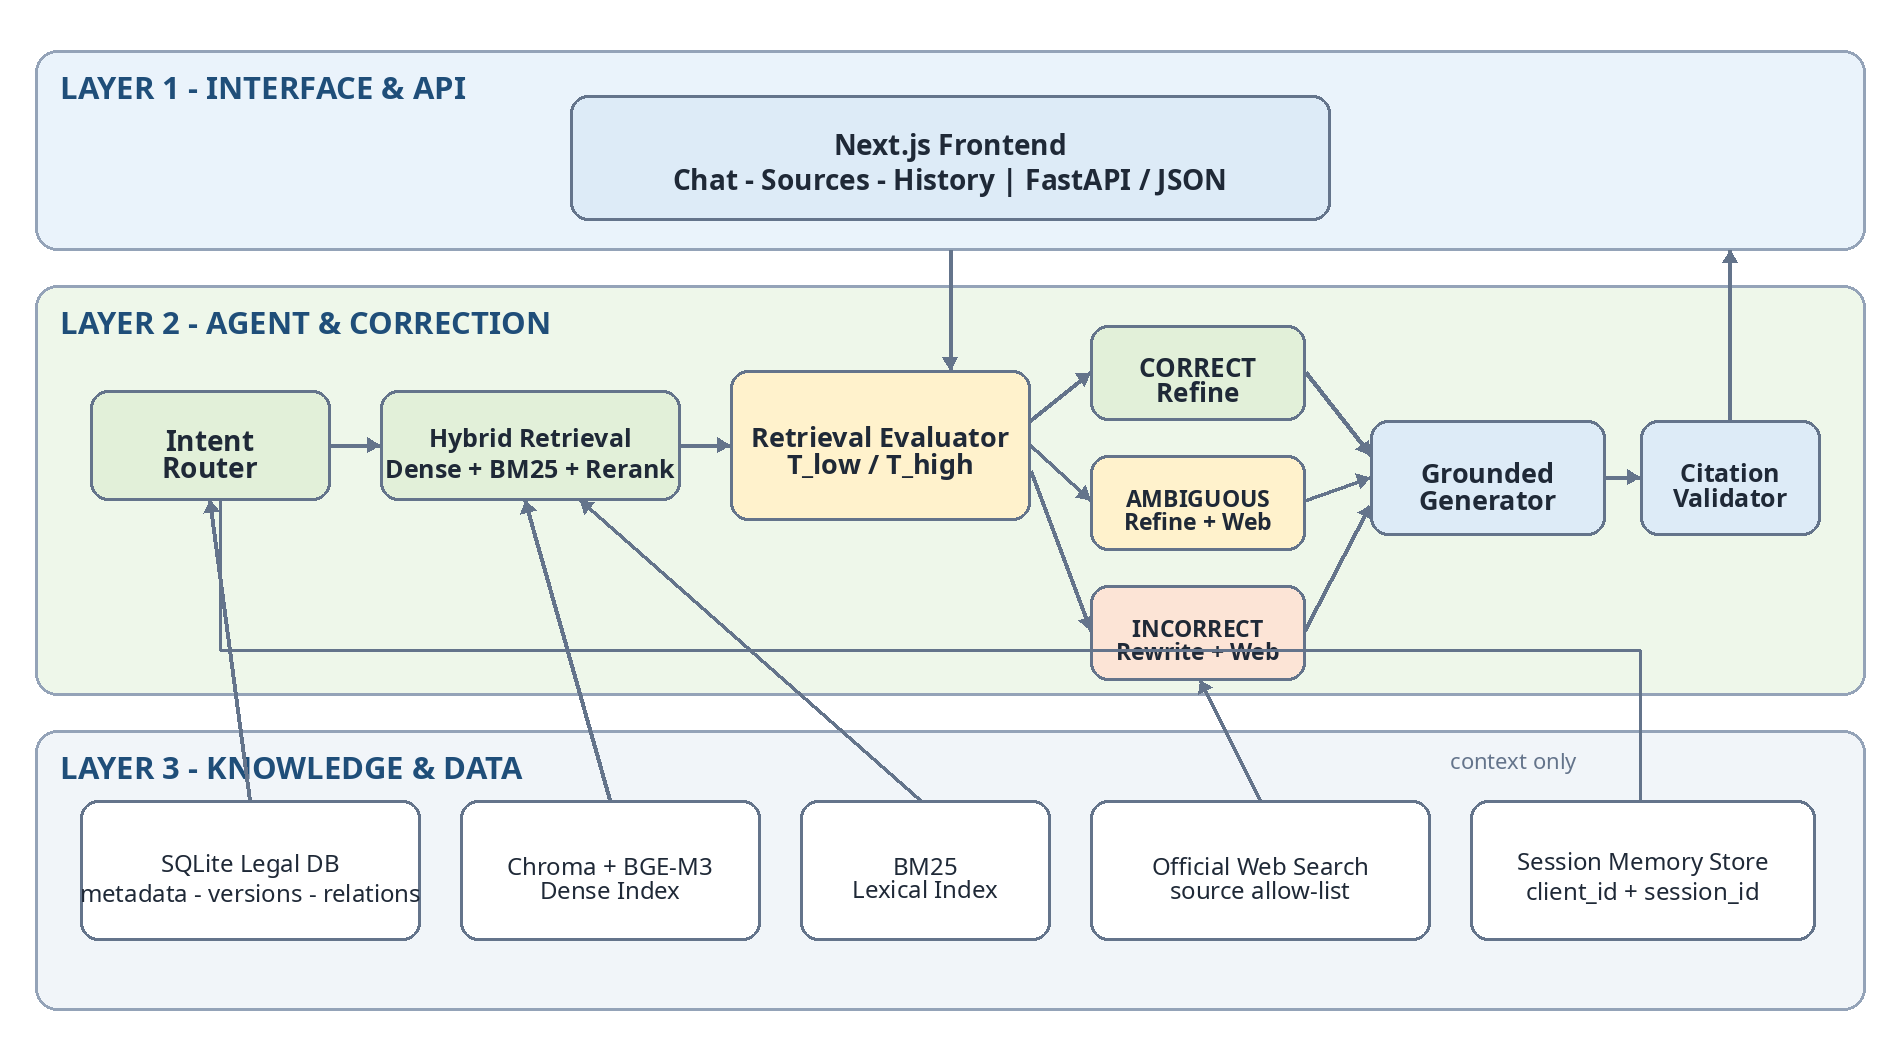
\includegraphics[width=0.92\textwidth]{images/figure_1.png}
    \caption{Kiến trúc 3 Layer của Legal CRAG Agent V3.}
    \label{fig:arch_3layer}
\end{figure}

\begin{table}[htbp]
\centering
\caption{Phân định chức năng và vai trò của từng Layer trong hệ thống}
\label{tab:layer_roles}
\renewcommand{\arraystretch}{1.3}
\rowcolors{2}{tablerowalt}{white}
\begin{tabularx}{\textwidth}{L{4.2cm} Y}
\toprule
\rowcolor{tableheader}\color{white}\textbf{Layer / Khối chức năng} & \color{white}\textbf{Vai trò và Trách nhiệm chính} \\
\midrule
\textbf{Layer 1 -- Interface \& API} & Next.js + TypeScript phụ trách giao diện người dùng chuyên nghiệp; FastAPI cung cấp hạ tầng RESTful/JSON API kết nối trực tiếp với Agent, hỗ trợ hiển thị câu trả lời, bảng trích dẫn citation, danh mục source và quản lý phiên. \\
\textbf{Layer 2 -- Agent \& Correction} & LangGraph điều phối toàn bộ workflow: Router phân loại câu hỏi, Retrieval Evaluator chấm điểm, 3 nhánh xử lý CRAG cốt lõi, Generator và Citation Validator đảm bảo độ chính xác. \\
\textbf{Layer 3 -- Knowledge \& Data} & SQLite quản lý metadata pháp lý và lịch sử phiên, Chroma DB lưu trữ dense vector index, BM25 lưu lexical index, Reranker tính toán relevance, và công cụ Controlled Web Search với danh sách nguồn cho phép. \\
\bottomrule
\end{tabularx}
\end{table}

\section{Luồng Hoạt động CRAG Cốt lõi (3 Nhánh)}

Trọng tâm của kỹ thuật Corrective RAG là không bao giờ tin tưởng tuyệt đối vào kết quả truy hồi ban đầu. Thay vào đó, một bộ đánh giá (\textit{Retrieval Evaluator}) sẽ phân loại tập tài liệu truy hồi thành một trong ba trạng thái:

\begin{figure}[htbp]
    \centering
    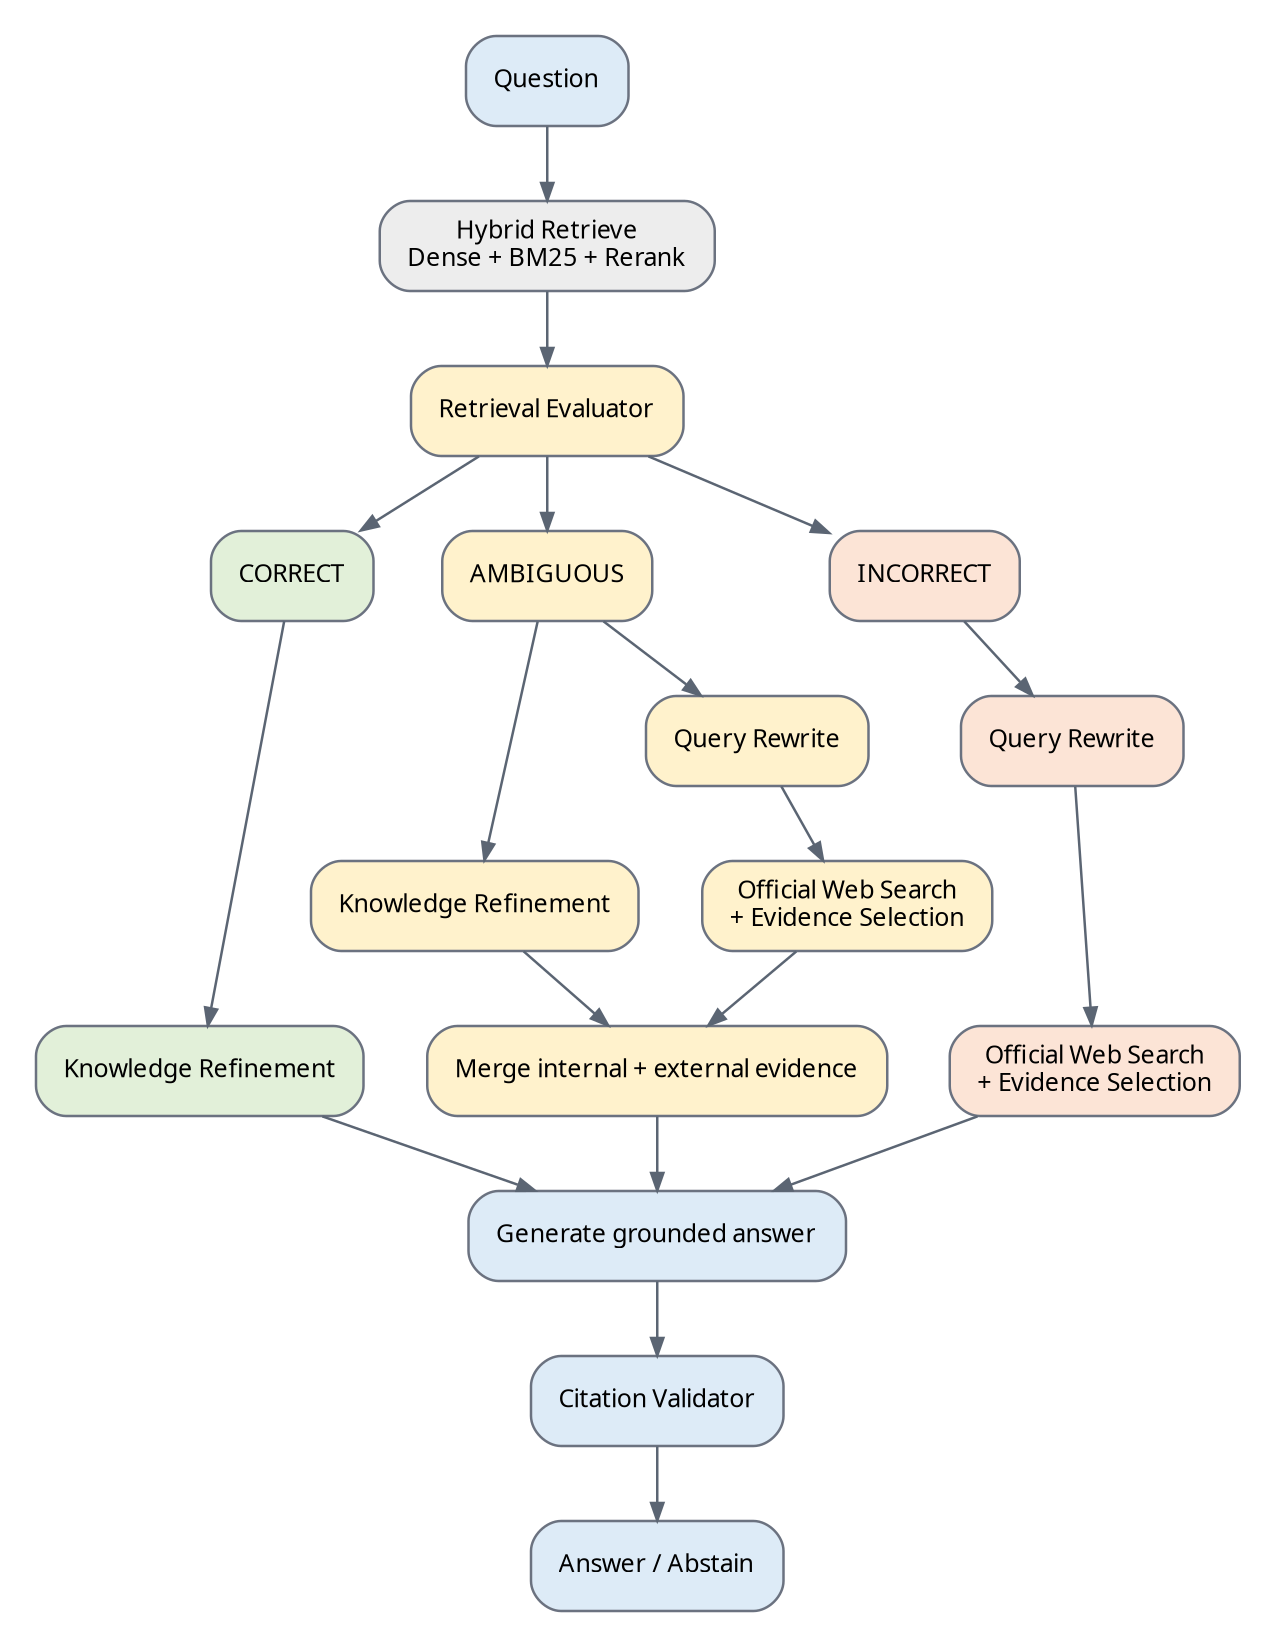
\includegraphics[width=0.75\textwidth]{images/figure_2.png}
    \caption{Luồng xử lý 3 nhánh Correct / Ambiguous / Incorrect theo nguyên lý CRAG.}
    \label{fig:crag_workflow}
\end{figure}

\begin{itemize}
    \item \textbf{Nhánh CORRECT (Tài liệu đạt chuẩn):} Điểm liên quan cao vượt ngưỡng $T_{high}$. Hệ thống kích hoạt \textit{Knowledge Refinement} để bóc tách các điều khoản (legal strips) trực tiếp trả lời câu hỏi, loại bỏ nhiễu và chuyển sang bộ sinh câu trả lời.
    \item \textbf{Nhánh INCORRECT (Tài liệu không phù hợp/thiếu hụt):} Điểm liên quan tối đa nằm dưới ngưỡng $T_{low}$. Hệ thống xác định corpus nội bộ không có căn cứ, loại bỏ toàn bộ tài liệu rác, thực hiện \textit{Query Rewrite} thành truy vấn tìm kiếm chuẩn mực và gọi công cụ \textit{Controlled Web Search} qua các cổng thông tin pháp luật chính thống.
    \item \textbf{Nhánh AMBIGUOUS (Tài liệu không rõ ràng/chưa đủ):} Điểm liên quan nằm giữa khoảng $[T_{low}, T_{high})$. Hệ thống vừa tinh chế tài liệu nội bộ, vừa viết lại truy vấn để tìm kiếm bổ sung trên web, sau đó tiến hành \textit{Evidence Merging} hợp nhất và khử trùng lặp trước khi sinh lời giải.
\end{itemize}

\begin{calloutbox}{Điểm cải tiến then chốt so với các thiết kế cũ}
Các phiên bản trước thường đưa nhánh \textit{Ambiguous} quay lại vòng lặp truy hồi (\textit{looping}) với biến \texttt{MAX\_ITER}. Thiết kế V3 loại bỏ việc lặp lại máy móc: nhánh Ambiguous bắt buộc phải kết hợp tinh lọc tri thức nội bộ và mở rộng nguồn web có kiểm soát, giải quyết dứt điểm vấn đề thiếu bằng chứng mà không gây lặp vô hạn.
\end{calloutbox}

\section{Stack Công nghệ Đề xuất}

\begin{table}[htbp]
\centering
\caption{Chi tiết Stack công nghệ triển khai hệ thống Legal CRAG V3}
\label{tab:tech_stack}
\renewcommand{\arraystretch}{1.25}
\rowcolors{2}{tablerowalt}{white}
\begin{tabularx}{\textwidth}{L{3.5cm} L{4.5cm} Y}
\toprule
\rowcolor{tableheader}\color{white}\textbf{Thành phần} & \color{white}\textbf{Công nghệ lựa chọn} & \color{white}\textbf{Lý do và Ghi chú kỹ thuật} \\
\midrule
Ngôn ngữ nền tảng & Python 3.11+ & Đảm bảo tính tương thích cao với LangGraph, PyTorch và transformers. \\
LLM Engine & Đa Provider (Groq, OpenAI, OpenRouter, Ollama) & Kiến trúc Factory linh hoạt: Groq (siêu tốc), OpenAI GPT-4o, OpenRouter và Ollama (local on-premise); cấu hình qua \texttt{LLM\_PROVIDER}; cố định \texttt{temperature=0}. \\
Embedding Model & BAAI/BGE-M3 & Embedding đa ngữ mạnh mẽ, xử lý tốt văn bản pháp luật tiếng Việt. \\
Dense Vector DB & ChromaDB & Nhẹ, nhúng trực tiếp, tối ưu cho quy mô 50--100 văn bản pháp lý. \\
Lexical Retrieval & rank-bm25 (BM25Okapi) & Bù đắp exact-match chính xác cho số hiệu văn bản, số Điều/Khoản. \\
Reranker & BAAI/bge-reranker-v2-m3 & Cross-encoder tính relevance score chuẩn xác cho Retrieval Evaluator. \\
Agent Orchestrator & LangGraph & Điều phối workflow dạng đồ thị có trạng thái (\textit{StateGraph}) và rẽ nhánh điều kiện. \\
Cơ sở dữ liệu & SQLite & Quản lý quan hệ văn bản, phiên bản điều luật, session logs và memory. \\
Web Search & Custom Engine + Allow-list & Chỉ thu thập từ các tên miền công quyền: \texttt{vbpl.vn}, \texttt{chinhphu.vn}... \\
Đánh giá chất lượng & RAGAS + Custom Metrics & Đo lường Faithfulness, Citation Accuracy và Legal Temporal Correctness. \\
Theo dõi & LangFuse & Ghi nhận toàn bộ vết thực thi, latency và chi phí token của từng node. \\
Frontend & Next.js + TypeScript & Giao diện tra cứu hiện đại, hiển thị bảng bằng chứng và lịch sử hội thoại. \\
API Gateway & FastAPI + Uvicorn & Cung cấp API chuẩn hóa REST/JSON kết nối UI và LangGraph Agent. \\
\bottomrule
\end{tabularx}
\end{table}

% !TEX root = ../main.tex
\chapter{Quy trình xây dựng hệ thống (18 bước hiện thực)}

\section{Bước 1: Chuẩn bị môi trường và cấu hình trung tâm}

Hệ thống yêu cầu cài đặt môi trường ảo riêng biệt sử dụng công cụ quản lý gói tốc độ cao \texttt{uv} trên nền tảng Python 3.13, cố định phiên bản các thư viện trước khi tiến hành thực nghiệm:

\begin{lstlisting}[language=bash, caption={Khởi tạo môi trường ảo và cài đặt các gói phụ thuộc}]
# Cai dat uv neu chua co tren he thong
curl -LsSf https://astral.sh/uv/install.sh | sh

# Khoi tao va kich hoat moi truong ao Python 3.13
uv venv --python 3.13 .venv
source .venv/bin/activate  # Tren macOS/Linux

# Cai dat cac goi thu vien phu thuoc
uv pip install langgraph langchain langchain-core langchain-community \
               langchain-chroma chromadb rank-bm25 FlagEmbedding \
               pypdf pymupdf beautifulsoup4 fastapi uvicorn[standard] \
               langfuse ragas datasets pydantic python-dotenv requests
\end{lstlisting}

Toàn bộ tham số vận hành được tập trung tại \texttt{config.py}, tránh ghi cứng rải rác trong mã nguồn:

\begin{lstlisting}[language=Python, caption={Cấu hình trung tâm hệ thống trong config.py}]
import os
from pathlib import Path

BASE_DIR = Path(__file__).resolve().parent
DB_PATH = BASE_DIR / "app.db"
CHROMA_DIR = BASE_DIR / "data" / "processed" / "chroma"

# Nha cung cap LLM: "groq" | "openai" | "openrouter" | "ollama"
LLM_PROVIDER = os.getenv("LLM_PROVIDER", "groq")
LLM_MODEL = os.getenv("LLM_MODEL", "llama-3.3-70b-versatile")
LLM_TEMPERATURE = 0.0

EMBEDDING_MODEL = "BAAI/bge-m3"
RERANKER_MODEL = "BAAI/bge-reranker-v2-m3"

TOP_K_DENSE = 20
TOP_K_BM25 = 20
TOP_K_RERANK = 5

# Cap nguong quyet dinh CRAG (Toi uu hoa qua thuc nghiem quet luoi)
T_LOW = 0.35
T_HIGH = 0.70
INTERNAL_STRIP_MIN = 0.40
MAX_TOOL_ROUNDS = 3
HISTORY_TURNS = 6
\end{lstlisting}

\section{Bước 2: Tổ chức thư mục dự án}

Mã nguồn được cấu trúc theo nguyên lý phân tách trách nhiệm rõ ràng, chia tách giữa tác tử hội thoại và quy trình nạp tri thức:

\begin{lstlisting}[language=bash, caption={Cấu trúc cây thư mục chuẩn hóa của Legal CRAG Assistant}]
crag/
├── agent/                     # Dieu phoi luot hoi thoai va vong lap ReAct
│   ├── graph.py               # Dinh nghia StateGraph, routing va bien dich do thi
│   ├── state.py               # Dinh nghia AgentState va cac reducer channels
│   ├── nodes.py               # Logic xu ly tai Agent Node, Tool Node, Validator
│   ├── runtime.py             # Diem vao duy nhat: prepare_turn, persist_turn
│   └── context.py             # Context Manager lap ghep lich su va ho so client
├── retrieval/                 # Engine truy hoi da phuong thuc va tinh che
│   ├── dense.py               # Truy hoi vector ChromaDB voi mo hinh BGE-M3
│   ├── bm25.py                # Truy hoi tu khoa chinh xac rank-bm25
│   ├── fusion.py              # Thuat toan hop nhat hang RRF k=60
│   ├── reranker.py            # Cross-Encoder Reranker va chuan hoa Sigmoid
│   └── refine.py              # Boc tach legal strips va loc nguong phap ly
├── tools/                     # Bo cong cu tac tu theo OpenAPI Schema
│   ├── base.py                # Lop co so BaseLegalTool
│   ├── registry.py            # Quan ly dang ky va phan phoi cong cu
│   ├── crag_search.py         # Cong cu CRAG noi bo (Hybrid Search + Refinement)
│   └── web_search.py          # Cong cu tim kiem web voi whitelist cong quyen
├── legal/                     # Xu ly chuyen biet van ban quy pham phap luat
│   ├── cleaner.py             # Lam sach Unicode NFC, bo dot leaders, headers
│   ├── parser.py              # Phan tach cau truc Chuong, Dieu, Khoan, Diem
│   ├── citations.py           # Bo kiem dinh trich dan xac dinh (Citation Validator)
│   └── temporal.py            # Kiem tra hieu luc van ban theo thoi gian thuc
├── memory/                    # Quan ly bo nho phien va ho so nguoi dung
│   ├── store.py               # SQLite storage cho sessions, messages, memories
│   └── extractor.py           # Trich xuat thuoc tinh doanh nghiep theo Allow-List
├── ingestion/                 # Pipeline nap tri thuc tu dong 8 giai doan
│   ├── worker.py              # Background Worker ThreadPool chay da luong
│   ├── chunks.py              # Giai thuat Legal-aware Chunking giu tron Dieu
│   └── indexer.py             # Dong bo hoa Chroma vector va chi muc BM25
├── eval/                      # Bo danh gia kiem chuan khoa hoc
│   ├── run_eval.py            # Script do benchmark tu dong tren tap test
│   ├── metrics.py             # Cong thuc tinh RAGAS, Fallback va Citation
│   └── benchmark_report.json  # Bao cao ket qua dinh luong thuc te
├── api/                       # Ha tang FastAPI RESTful va SSE streaming
├── frontend/                  # Ung dung giao dien Next.js 14 SPA
├── schema.sql                 # DDL 8 bang quan he SQLite canonical
└── config.py                  # Cau hinh tham so tap trung toan he thong
\end{lstlisting}

\section{Bước 3: Chuẩn bị dữ liệu quy phạm pháp luật}

Dữ liệu được thu thập có chọn lọc từ Cổng Thông tin Điện tử Chính phủ (\texttt{chinhphu.vn}) và Cơ sở Dữ liệu Quốc gia về Văn bản Pháp luật (\texttt{vbpl.vn}), tập trung vào Luật Doanh nghiệp 2020, Bộ luật Lao động 2019 và các văn bản sửa đổi, bổ sung liên quan.

\begin{table}[htbp]
\centering
\caption{Quy mô dữ liệu quy phạm và các tập kiểm thử trong hệ thống}
\label{tab:corpus_scale}
\renewcommand{\arraystretch}{1.25}
\rowcolors{2}{tablerowalt}{white}
\begin{tabularx}{\textwidth}{L{6.0cm} Y}
\toprule
\rowcolor{tableheader}\color{white}\textbf{Thành phần dữ liệu} & \color{white}\textbf{Quy mô thực tế} \\
\midrule
Tổng số văn bản quy phạm thu thập & 27 văn bản (Luật, Nghị định, Thông tư, Văn bản hợp nhất) \\
Văn bản đã qua quy trình nạp đạt trạng thái READY & 15 văn bản chuẩn hóa hoàn chỉnh \\
Tổng số đoạn trích phân đoạn pháp lý (\textit{document\_chunks}) & 1.067 đoạn trích có tiêu đề ngữ cảnh \\
Tập dữ liệu hiệu chuẩn ngưỡng (\textit{Calibration Set}) & 20 câu hỏi có gán nhãn sự thật khách quan \\
Tập kiểm thử độc lập (\textit{Held-out Test Set}) & 40 câu hỏi phân bổ đều theo 5 nhóm nghiệp vụ \\
\bottomrule
\end{tabularx}
\end{table}

\section{Bước 4 \& 5: Thiết kế và khởi tạo cơ sở dữ liệu pháp lý SQLite}

Toàn bộ mô hình dữ liệu quan hệ được định nghĩa trong \texttt{schema.sql}, gồm 8 bảng phân chia giữa phân hệ nạp tri thức và phân hệ hội thoại:

\begin{lstlisting}[language=SQL, caption={Trích đoạn DDL lược đồ cơ sở dữ liệu SQLite app.db}]
PRAGMA foreign_keys = ON;

-- 1. Quan ly danh muc van ban phap ly goc
CREATE TABLE IF NOT EXISTS documents (
    id TEXT PRIMARY KEY,
    filename TEXT NOT NULL,
    document_number TEXT,
    title TEXT NOT NULL,
    document_type TEXT,
    issuing_authority TEXT,
    effective_from DATE,
    effective_to DATE,
    status TEXT NOT NULL DEFAULT 'UPLOADED', -- UPLOADED | PROCESSING | READY | FAILED
    legal_status TEXT NOT NULL DEFAULT 'effective', -- effective | expired | partially_expired
    content_hash TEXT,
    chunk_count INTEGER DEFAULT 0,
    created_at TEXT DEFAULT CURRENT_TIMESTAMP
);

-- 2. Cac doan trich phan manh phap ly (don vi truy hoi co so)
CREATE TABLE IF NOT EXISTS document_chunks (
    id TEXT PRIMARY KEY,
    document_id TEXT NOT NULL,
    chunk_index INTEGER NOT NULL,
    chapter TEXT, article TEXT, clause TEXT, point TEXT,
    heading TEXT,
    page_start INTEGER, page_end INTEGER,
    content TEXT NOT NULL,
    token_count INTEGER,
    FOREIGN KEY(document_id) REFERENCES documents(id) ON DELETE CASCADE
);

-- 3. Quan he sua doi, bo sung, thay the giua cac van ban
CREATE TABLE IF NOT EXISTS legal_relations (
    id INTEGER PRIMARY KEY AUTOINCREMENT,
    source_document_id TEXT NOT NULL,
    target_document_id TEXT NOT NULL,
    relation_type TEXT NOT NULL, -- 'amends', 'supplements', 'replaces', 'repeals', 'guides'
    note TEXT,
    FOREIGN KEY(source_document_id) REFERENCES documents(id) ON DELETE CASCADE,
    FOREIGN KEY(target_document_id) REFERENCES documents(id) ON DELETE CASCADE
);

-- 4. Tien trinh xu ly nap du lieu cua quan tri vien
CREATE TABLE IF NOT EXISTS ingestion_jobs (
    id TEXT PRIMARY KEY,
    document_id TEXT NOT NULL,
    stage TEXT NOT NULL DEFAULT 'PARSING',
    progress REAL NOT NULL DEFAULT 0.0,
    detail TEXT,
    FOREIGN KEY(document_id) REFERENCES documents(id) ON DELETE CASCADE
);
\end{lstlisting}

\section{Bước 6: Cấu hình LLM đa nhà cung cấp, mô hình nhúng và xếp hạng lại}

Module \texttt{llm.py} cài đặt mô hình Factory Pattern hỗ trợ đa nhà cung cấp, đảm bảo tính sẵn sàng cao với cơ chế chuyển đổi dự phòng tự động:

\begin{lstlisting}[language=Python, caption={Khởi tạo mô hình ngôn ngữ, mô hình nhúng và xếp hạng lại}]
# llm.py
from config import LLM_PROVIDER, LLM_MODEL, LLM_TEMPERATURE

def get_chat_model(provider: str = None, model: str = None):
    p = (provider or LLM_PROVIDER).lower()
    m = model or LLM_MODEL
    if p == "groq":
        from langchain_groq import ChatGroq
        return ChatGroq(model=m, temperature=LLM_TEMPERATURE)
    elif p == "openai":
        from langchain_openai import ChatOpenAI
        return ChatOpenAI(model=m, temperature=LLM_TEMPERATURE)
    elif p == "ollama":
        from langchain_ollama import ChatOllama
        return ChatOllama(model=m, temperature=LLM_TEMPERATURE)
    # OpenRouter va logic chuyen doi du phong...

# Khoi tao mo hinh nhung da ngu BAAI/bge-m3 (vector 1024 chieu)
from langchain_ollama import OllamaEmbeddings
embeddings = OllamaEmbeddings(model="bge-m3")

# retrieval/reranker.py: Mo hinh Cross-Encoder BAAI/bge-reranker-v2-m3
from FlagEmbedding import FlagReranker
from math import exp

reranker = FlagReranker("BAAI/bge-reranker-v2-m3", use_fp16=True)

def sigmoid(z: float) -> float:
    return 1.0 / (1.0 + exp(-float(z)))

def rerank(query: str, docs: list[dict], top_k: int = 5) -> list[dict]:
    if not docs:
        return []
    pairs = [[query, d.get("content", d.get("text", ""))] for d in docs]
    raw_scores = reranker.compute_score(pairs)
    scored = []
    for doc, s in zip(docs, raw_scores):
        doc_copy = dict(doc)
        doc_copy["score"] = sigmoid(s)
        scored.append(doc_copy)
    return sorted(scored, key=lambda x: x["score"], reverse=True)[:top_k]
\end{lstlisting}

\section{Bước 7: Định nghĩa trạng thái tác tử với các bộ tích lũy}

Để duy trì quỹ đạo ReAct nhiều lượt và thu thập chứng cứ không bị ghi đè, \texttt{AgentState} được định nghĩa với các bộ tích lũy chuyên dụng:

\begin{lstlisting}[language=Python, caption={Định nghĩa trạng thái AgentState trong agent/state.py}]
import operator
from typing import Annotated, Any, Dict, List, Optional, TypedDict
from langchain_core.messages import BaseMessage
from langgraph.graph.message import add_messages

class AgentState(TypedDict, total=False):
    # Thong tin yeu cau va ngu canh hoi thoai
    client_id: str
    session_id: str
    query: str
    as_of_date: Optional[str]
    memory_context: str
    conversation_history: str

    # Quy dao suy luan ReAct (Tich luy qua cac luot goi cong cu)
    messages: Annotated[List[BaseMessage], add_messages]
    evidence: Annotated[List[Dict[str, Any]], operator.add]
    tool_trace: Annotated[List[Dict[str, Any]], operator.add]

    # Ket qua sinh va kiem dinh trich dan
    generation: Dict[str, Any]       # {"answer": str, "claims": [...], "abstain": bool}
    citation_report: Dict[str, Any]  # Ket qua tu CitationValidator
    follow_up_questions: List[str]   # Goi y cau hoi tiep theo
    trace_meta: Dict[str, Any]
\end{lstlisting}

\section{Bước 8: Quy trình nạp dữ liệu và phân đoạn pháp lý}

Quy trình nạp tài liệu tự động gồm 8 giai đoạn khép kín, được minh họa chi tiết tại Hình~\ref{fig:ingestion_pipeline}.

\begin{figure}[htbp]
    \centering
    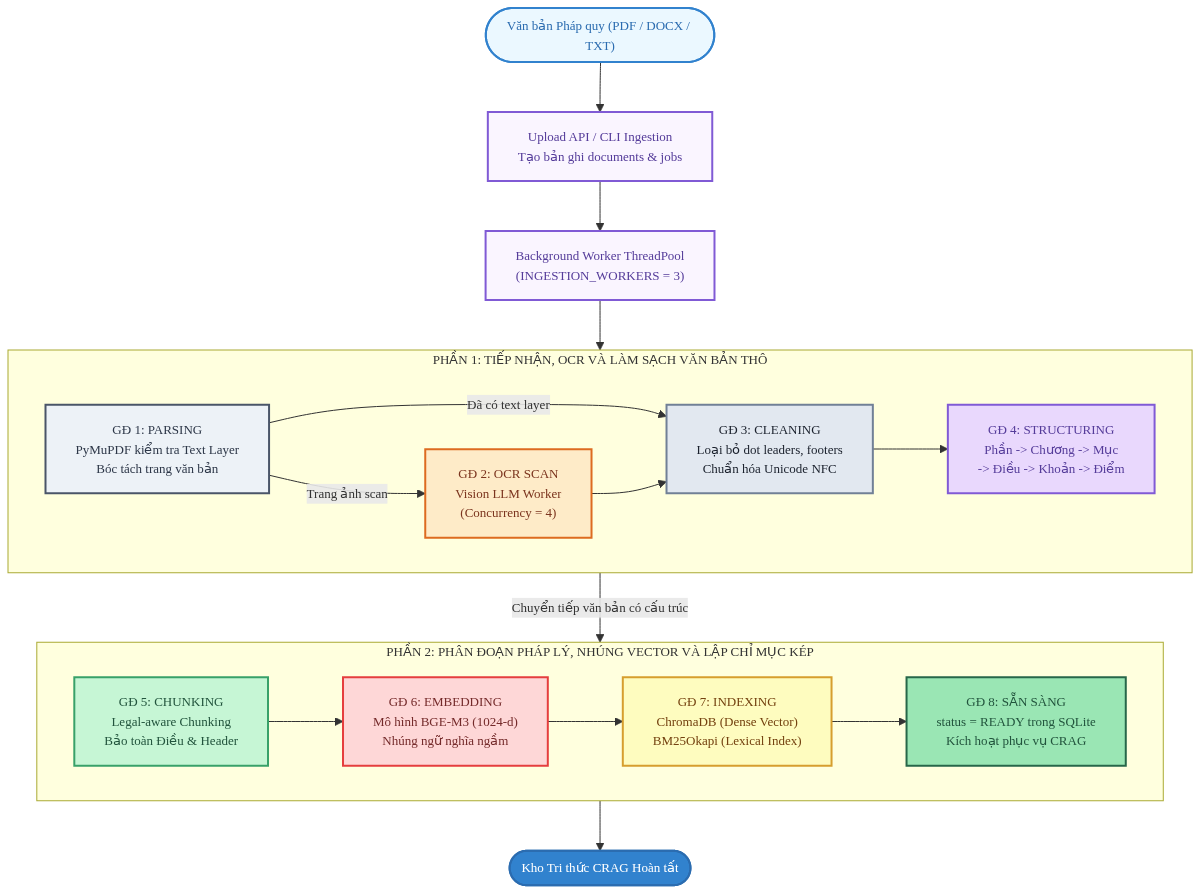
\includegraphics[width=\textwidth]{images/ingestion_pipeline.png}
    \caption{Quy trình 8 giai đoạn nạp dữ liệu tự động từ tệp văn bản thô đến chỉ mục kép Chroma và BM25.}
    \label{fig:ingestion_pipeline}
\end{figure}

Tiến trình xử lý được chia thành:
\begin{enumerate}
    \item \textbf{Phân tích cú pháp và nhận dạng quang học:} Nhận diện tệp Word hoặc PDF. Các trang quét ảnh scan được bóc tách và nạp qua Vision LLM OCR với mức song song $\text{OCR\_CONCURRENCY} = 4$.
    \item \textbf{Làm sạch và cấu trúc hóa:} Loại bỏ biểu mẫu chấm, tiêu đề đầu trang và chân trang, chuẩn hóa bảng mã Unicode tiếng Việt NFC và nhận diện thứ bậc quy phạm pháp luật (\textit{Phần $\to$ Chương $\to$ Mục $\to$ Điều $\to$ Khoản $\to$ Điểm}).
    \item \textbf{Phân đoạn pháp lý bảo toàn ngữ cảnh:} Phân đoạn ngữ nghĩa điều luật bảo toàn ranh giới (Hình~\ref{fig:legal_chunking_flow}).
    \item \textbf{Nhúng vector và lập chỉ mục:} Tạo vector ngữ nghĩa BGE-M3 lưu vào ChromaDB và cập nhật chỉ mục từ khóa BM25Okapi dưới nền.
\end{enumerate}

\begin{figure}[htbp]
    \centering
    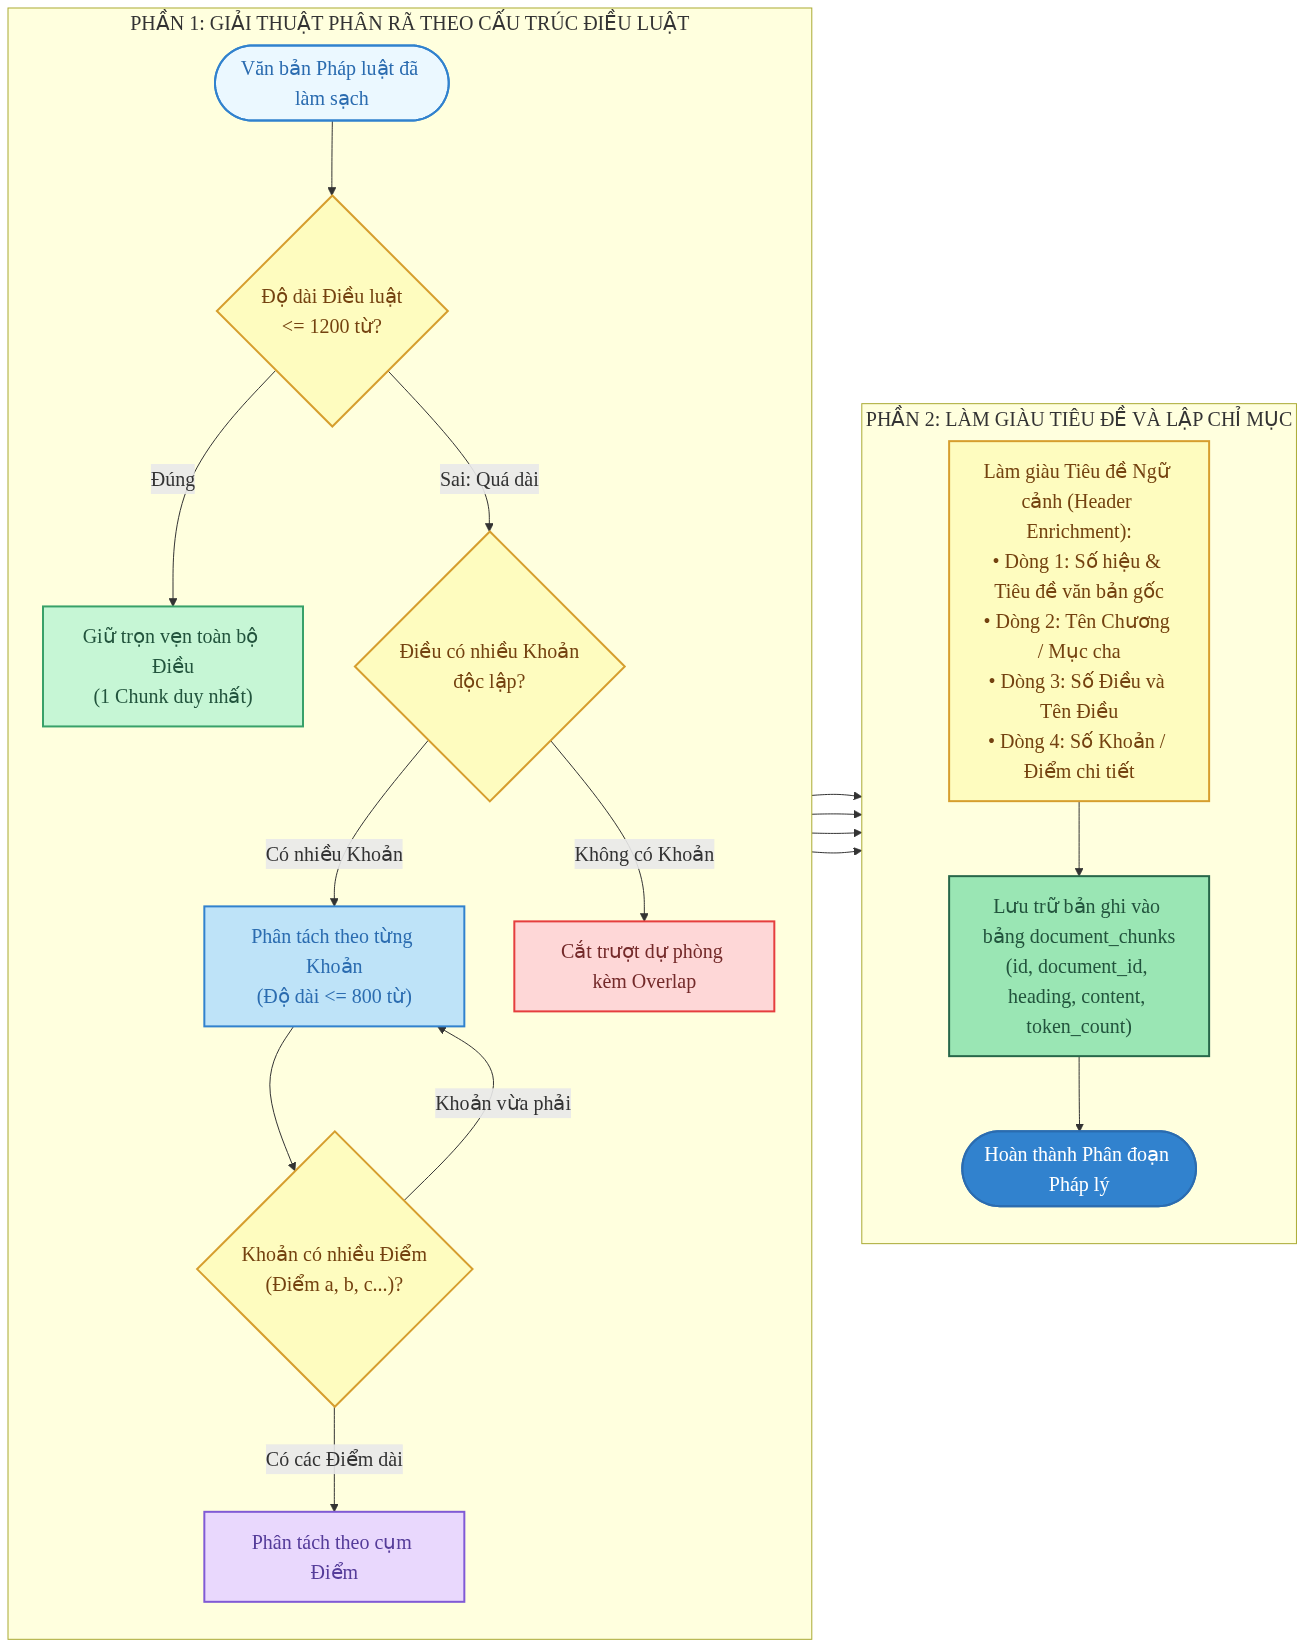
\includegraphics[width=0.88\textwidth]{images/legal_chunking_flow.png}
    \caption{Giải thuật phân đoạn pháp lý Legal-aware Chunking: Bảo toàn nguyên vẹn Điều luật và làm giàu tiêu đề ngữ cảnh.}
    \label{fig:legal_chunking_flow}
\end{figure}

Giải thuật phân đoạn pháp lý tuân thủ nguyên tắc:
\begin{itemize}
    \item Nếu Điều luật $\le 1200$ từ: Giữ nguyên vẹn toàn bộ Điều thành một đoạn trích duy nhất nhằm bảo toàn tính thống nhất giữa các khoản quy định.
    \item Nếu Điều luật $> 1200$ từ: Phân tách theo từng Khoản độc lập; nếu Khoản vẫn quá dài thì tiếp tục bóc tách theo cụm Điểm.
    \item \textbf{Làm giàu tiêu đề ngữ cảnh:} Mỗi đoạn trích đều được gắn kèm dòng tiêu đề ngữ cảnh phân cấp: \textit{Số hiệu văn bản $\to$ Tên Chương/Mục $\to$ Tên Điều $\to$ Số Khoản/Điểm}.
\end{itemize}

\section{Bước 9: Hệ thống quản trị công cụ và cơ chế điều phối}

Module \texttt{tools/registry.py} quản lý danh mục công cụ, chuyển đổi tự động sang cấu trúc lược đồ chuẩn để mô hình ngôn ngữ lớn thực hiện cơ chế gọi hàm (\textit{function calling}) một cách chuẩn xác.

\section{Bước 10: Động cơ truy hồi CRAG và bộ đánh giá ba nhánh}

Công cụ \texttt{crag\_search} là trọng tâm của kỹ thuật Corrective RAG trong hệ thống, thực hiện quy trình xử lý khép kín mô tả tại Hình~\ref{fig:crag_retrieval_branches}.

\begin{figure}[htbp]
    \centering
    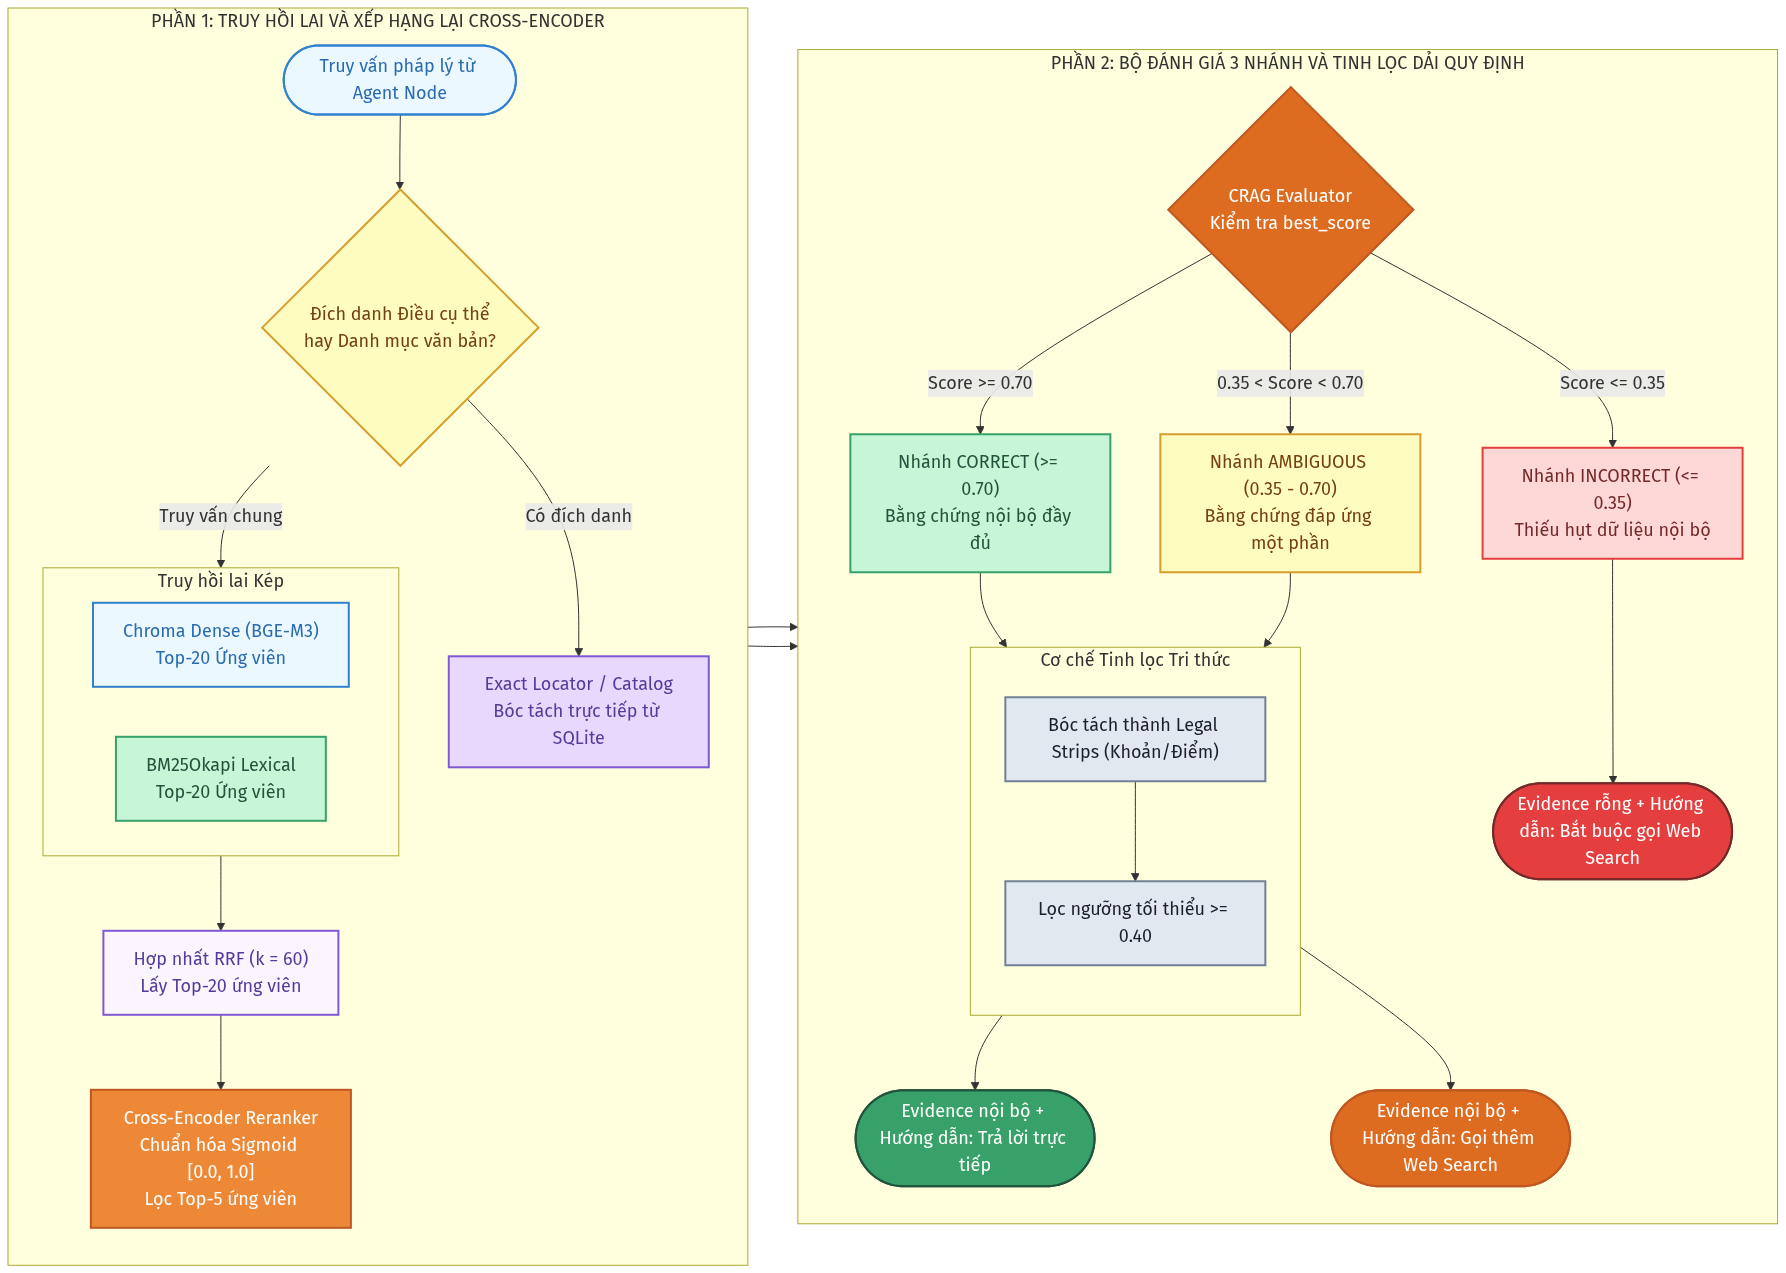
\includegraphics[width=\textwidth]{images/crag_retrieval_branches.png}
    \caption{Luồng xử lý chi tiết bên trong công cụ crag\_search và cơ chế rẽ ba nhánh điều kiện của CRAG.}
    \label{fig:crag_retrieval_branches}
\end{figure}

\subsection{Truy hồi lai và hợp nhất thứ hạng RRF}
Hệ thống truy hồi đồng thời 20 ứng viên hàng đầu từ Chroma (Dense) và 20 ứng viên từ BM25 (Lexical), sau đó hợp nhất bằng giải thuật Reciprocal Rank Fusion với hằng số làm mịn $k = 60$:
\begin{equation}
S_{\text{RRF}}(d) = \sum_{r \in \{\text{Dense}, \text{BM25}\}} \frac{1}{60 + \text{rank}_r(d)}
\end{equation}

\subsection{Đánh giá và rẽ ba nhánh điều kiện CRAG}
Danh sách 5 ứng viên hàng đầu sau khi xếp hạng lại bằng Cross-Encoder được đưa qua hàm đánh giá ngưỡng:
\begin{equation}
\text{Action} = \begin{cases}
\mathbf{CORRECT} & \text{nếu } \max(S) \ge T_{high} \;(0.70) \\
\mathbf{INCORRECT} & \text{nếu } \max(S) \le T_{low} \;(0.35) \\
\mathbf{AMBIGUOUS} & \text{nếu } T_{low} < \max(S) < T_{high}
\end{cases}
\end{equation}

\subsection{Cơ chế tinh lọc tri thức (Knowledge Refinement)}
Khi nhánh rẽ là \textbf{CORRECT} hoặc \textbf{AMBIGUOUS}, hệ thống kích hoạt \texttt{refine\_internal}:
\begin{enumerate}
    \item Phân rã từng đoạn văn bản thành các dải quy định cụ thể (\textit{legal strips} theo từng Khoản hoặc Điểm).
    \item Chấm lại điểm liên quan của từng dải quy định bằng mô hình Cross-Encoder.
    \item Lọc bỏ toàn bộ các dải quy định có điểm số dưới ngưỡng tối thiểu $\text{INTERNAL\_STRIP\_MIN} = 0.40$.
\end{enumerate}

\section{Bước 11: Tìm kiếm web có kiểm soát}

Khi kho dữ liệu nội bộ không có căn cứ phù hợp (\textbf{INCORRECT}) hoặc chỉ đáp ứng một phần (\textbf{AMBIGUOUS}), tác tử tự động gọi công cụ tìm kiếm web với danh mục tên miền cho phép:
\begin{lstlisting}[language=Python, caption={Bộ lọc tên miền chính thống cho công cụ tìm kiếm web}]
OFFICIAL_DOMAINS = {
    "vbpl.vn", "vanban.chinhphu.vn", "moj.gov.vn", 
    "chinhphu.vn", "thuvienphapluat.vn", "congbao.chinhphu.vn"
}

def is_allowed_source(url: str) -> bool:
    try:
        host = url.lower().split("/")[2]
        return any(host == d or host.endswith("." + d) for d in OFFICIAL_DOMAINS)
    except Exception:
        return False
\end{lstlisting}

\section{Bước 12: Bộ kiểm định trích dẫn xác định}

Module \texttt{legal/citations.py} đóng vai trò chốt chặn an toàn cuối cùng trước khi phản hồi được xuất ra cho người dùng:
\begin{enumerate}
    \item \textbf{Kiểm tra tính tồn tại của căn cứ:} Mọi mã trích dẫn \texttt{[source\_id]} xuất hiện trong câu trả lời phải nằm trong tập bằng chứng (\textit{evidence map}) đã được thu thập thực tế.
    \item \textbf{Kiểm tra tính hiệu lực theo thời gian:} Căn cứ vào ngày tham chiếu \texttt{as\_of\_date}, hệ thống đối chiếu với trường \texttt{effective\_from}, \texttt{effective\_to} và quan hệ bãi bỏ/thay thế trong cơ sở dữ liệu để cảnh báo nếu trích dẫn văn bản đã hết hiệu lực.
    \item \textbf{Cơ chế từ chối an toàn (Safe Abstain):} Nếu phát hiện trích dẫn giả mạo hoặc không có căn cứ, hệ thống tự động gắn cờ \texttt{abstain = true} và thay thế bằng câu trả lời an toàn chuẩn: \textit{“Chưa đủ căn cứ pháp lý để kết luận.”}
\end{enumerate}

\section{Bước 13: Thiết kế câu lệnh nhắc sinh phản hồi có cấu trúc JSON}

Mô hình ngôn ngữ được ràng buộc tuân thủ khuôn dạng đầu ra có cấu trúc nhằm phân tách rõ rệt giữa mệnh đề kết luận và mã nguồn trích dẫn:

\begin{lstlisting}[caption={Câu lệnh nhắc sinh câu trả lời có cấu trúc nghiêm ngặt}]
Bạn là trợ lý hỗ trợ tra cứu tuân thủ pháp lý doanh nghiệp.
Chỉ trả lời dựa duy nhất trên các căn cứ pháp lý hiện tại được cung cấp dưới đây.

Yêu cầu bắt buộc:
1. Tuyệt đối không tự suy đoán hoặc sáng tạo quy định pháp luật.
2. Mọi kết luận pháp lý phải được gắn kèm [source_id] của bằng chứng tương ứng.
3. Nếu chưa đủ căn cứ, trả lời rõ ràng: "Chưa đủ căn cứ pháp lý để kết luận."
4. Định dạng đầu ra: Bắt buộc trả về đúng định dạng JSON Schema:
   {
     "answer": "Nội dung giải thích súc tích...",
     "claims": [
       {"text": "Mệnh đề pháp lý 1", "source_ids": ["E1", "E2"]},
       {"text": "Mệnh đề pháp lý 2", "source_ids": ["E3"]}
     ],
     "abstain": false
   }

Căn cứ pháp lý:
{evidence_context}

Câu hỏi:
{query}
\end{lstlisting}

\section{Bước 14: Xây dựng và biên dịch đồ thị LangGraph ReAct}

Lõi điều phối được lập trình trong \texttt{agent/graph.py} với đồ thị trạng thái 3 nút chính:

\begin{lstlisting}[language=Python, caption={Thiết lập đồ thị LangGraph ReAct trong agent/graph.py}]
from langgraph.graph import StateGraph, START, END
from agent.state import AgentState
from agent.nodes import agent_node, route_after_agent, tool_node, validate_citations_node

def build_crag_graph():
    g = StateGraph(AgentState)
    
    # Ba nut chinh cua chu trinh ReAct
    g.add_node("agent", agent_node)
    g.add_node("tools", tool_node)
    g.add_node("cite_validate", validate_citations_node)
    
    g.add_edge(START, "agent")
    
    # Canh dieu kien phan nhanh sau khi Agent suy luan
    g.add_conditional_edges(
        "agent",
        route_after_agent,
        {
            "tools": "tools",                   # LLM yeu cau goi cong cu
            "agent": "agent",                   # Tiep tuc suy luan
            "cite_validate": "cite_validate"    # Hoan tat, chuyen sang kiem dinh
        }
    )
    
    g.add_edge("tools", "agent")                # Observation tra ve cho Agent
    g.add_edge("cite_validate", END)            # Ket thuc luot hoi thoai
    
    return g.compile()
\end{lstlisting}

\section{Bước 15: Kịch bản kiểm thử thực nghiệm phục vụ trình diễn}

Hệ thống cung cấp sẵn kịch bản kiểm thử tự động \texttt{python main.py --demo} bao phủ 5 tình huống kiểm thử đại diện (Bảng~\ref{tab:demo_tests}).

\begin{table}[htbp]
\centering
\caption{Năm kịch bản kiểm thử bắt buộc cần minh chứng hoạt động của CRAG}
\label{tab:demo_tests}
\renewcommand{\arraystretch}{1.25}
\rowcolors{2}{tablerowalt}{white}
\begin{tabularx}{\textwidth}{C{1.8cm} L{4.0cm} Y}
\toprule
\rowcolor{tableheader}\color{white}\textbf{Kịch bản} & \color{white}\textbf{Tình huống kiểm thử} & \color{white}\textbf{Luồng xử lý kỳ vọng của hệ thống} \\
\midrule
\textbf{Kịch bản 1} & \textit{Correct Case:} Câu hỏi trong kho có đầy đủ căn cứ nội bộ. & Điểm số $\ge 0.70 \;\to\; \mathbf{CORRECT} \;\to\; \text{Tinh lọc dải quy định} \;\to\; \text{Sinh phản hồi} \;\to\; \text{Kiểm định trích dẫn}$. \\
\textbf{Kịch bản 2} & \textit{Incorrect Case:} Câu hỏi về nghị định mới chưa nạp vào kho dữ liệu. & Điểm số $\le 0.35 \;\to\; \mathbf{INCORRECT} \;\to\; \text{Viết lại truy vấn} \;\to\; \text{Tìm kiếm web chính thống} \;\to\; \text{Sinh phản hồi}$. \\
\textbf{Kịch bản 3} & \textit{Ambiguous Case:} Kho nội bộ có quy định khung nhưng thiếu thủ tục chi tiết. & $0.35 < \text{Điểm} < 0.70 \;\to\; \mathbf{AMBIGUOUS} \;\to\; \text{Tinh lọc} + \text{Web} \;\to\; \text{Hợp nhất bằng chứng} \;\to\; \text{Sinh phản hồi}$. \\
\textbf{Kịch bản 4} & \textit{Exact Locator:} “Điều 25 Bộ luật Lao động 2019 quy định gì?” & Cơ chế định vị trực tiếp bóc tách toàn bộ các Khoản từ SQLite $\;\to\;$ Phản hồi chính xác tuyệt đối. \\
\textbf{Kịch bản 5} & \textit{Citation Guardrail:} Mô hình cố tình trích dẫn nguồn không có thật. & Bộ kiểm định phát hiện mã trích dẫn giả mạo $\;\to\;$ Thiết lập \texttt{abstain = true} chặn đứng ảo giác. \\
\bottomrule
\end{tabularx}
\end{table}

% !TEX root = ../main.tex
\chapter{Thiết kế Thực nghiệm \& Đánh giá Hệ thống}

\section{Thiết kế Hệ thống Baseline và Nghiên cứu Ablation}

Để chứng minh tính vượt trội của Corrective RAG ở chuẩn mực nghiên cứu cao học, không thể chỉ so sánh đơn thuần giữa Traditional RAG và Full CRAG. Cần xây dựng các hệ thống đối chứng để phân tách rạch ròi: \textit{Sự cải thiện đến từ cơ chế hiệu chỉnh tri thức hay chỉ đơn thuần do hệ thống được cấp thêm nguồn Web bên ngoài?}

\begin{table}[htbp]
\centering
\caption{Ma trận các hệ thống Baseline thực nghiệm (S0 -- S4)}
\label{tab:baselines}
\renewcommand{\arraystretch}{1.25}
\rowcolors{2}{tablerowalt}{white}
\begin{tabularx}{\textwidth}{C{1.8cm} C{2.2cm} C{2.5cm} C{2.5cm} Y}
\toprule
\rowcolor{tableheader}\color{white}\textbf{Hệ thống} & \color{white}\textbf{Evaluator} & \color{white}\textbf{Web Search} & \color{white}\textbf{Correction} & \color{white}\textbf{Mục đích nghiên cứu} \\
\midrule
\textbf{S0} & Không & Không & Không & LLM-only: Đo lường tri thức nội tại của mô hình, làm mốc tham chiếu không retrieval. \\
\textbf{S1} & Không & Không & Không & Traditional RAG: Truy hồi Top-K cố định đưa thẳng vào Generator. \\
\textbf{S2} & Không & Luôn luôn & Không & RAG + Always Web: Luôn tìm kiếm web để tách riêng hiệu ứng “có thêm nguồn ngoài”. \\
\textbf{S3} & Có & Không & Một phần & RAG + Evaluator: Đánh giá bằng chứng nhưng chỉ quyết định trả lời hoặc từ chối (\textit{abstain}). \\
\textbf{S4} & Có & Có điều kiện & Toàn diện & \textbf{Full CRAG đề xuất:} Đầy đủ 3 nhánh Correct, Ambiguous và Incorrect. \\
\bottomrule
\end{tabularx}
\end{table}

\begin{infobox}{Các Biến thể Ablation Study Khuyến nghị}
\begin{itemize}
    \item \textbf{Ablation 1 (No Refinement):} Full CRAG loại bỏ bước Knowledge Refinement (đưa nguyên chunk dài vào Generator).
    \item \textbf{Ablation 2 (No Rewrite):} Full CRAG loại bỏ Query Rewrite (dùng trực tiếp câu hỏi thô để search web).
    \item \textbf{Ablation 3 (No Web Selection):} Lấy nguyên trang web fetch được mà không qua bộ lọc relevance strip.
    \item \textbf{Ablation 4 (Dense-only):} Thay thế Hybrid Retrieval bằng truy hồi vector thuần túy BGE-M3.
    \item \textbf{Ablation 5 (No Reranker):} Bỏ mô hình Cross-Encoder, dùng trực tiếp similarity score của vector để routing.
\end{itemize}
\end{infobox}

\section{Thiết kế Tập Calibration và Held-Out Test Set}

\begin{calloutbox}{Quy tắc vàng trong đánh giá học thuật}
Tuyệt đối không sử dụng cùng một tập dữ liệu vừa để tìm ngưỡng $T_{low}/T_{high}$ vừa để báo cáo kết quả cuối cùng. Hệ thống phải tách biệt nghiêm ngặt hai tập dữ liệu độc lập:
\end{calloutbox}

\begin{table}[htbp]
\centering
\caption{Phân bổ các nhóm câu hỏi trong Held-out Test Set (40 câu)}
\label{tab:test_set_distribution}
\renewcommand{\arraystretch}{1.25}
\rowcolors{2}{tablerowalt}{white}
\begin{tabularx}{\textwidth}{L{5cm} C{2cm} Y}
\toprule
\rowcolor{tableheader}\color{white}\textbf{Nhóm câu hỏi kiểm thử} & \color{white}\textbf{Số lượng} & \color{white}\textbf{Mục tiêu kiểm chứng} \\
\midrule
Correct / In-corpus & 12 câu & Bằng chứng nội bộ đầy đủ, kiểm tra hiệu quả của Knowledge Refinement. \\
Incorrect / Out-of-corpus & 10 câu & Corpus nội bộ thiếu hụt, kiểm tra khả năng kích hoạt Web Search chính thống. \\
Ambiguous / Partial evidence & 8 câu & Kiểm tra cơ chế hợp nhất tri thức nội bộ và tri thức mở rộng bên ngoài. \\
Metadata / Database queries & 5 câu & Đo lường độ chính xác của Router và khả năng truy vấn dữ liệu có cấu trúc. \\
Temporal / Conflicting sources & 5 câu & Kiểm tra khả năng phát hiện văn bản hết hiệu lực và giải quyết xung đột điều luật. \\
\midrule
\textbf{Tổng cộng} & \textbf{40 câu} & \textbf{Tập dữ liệu độc lập hoàn toàn, khóa trước khi đo benchmark.} \\
\bottomrule
\end{tabularx}
\end{table}

Mỗi mẫu trong tập kiểm thử được lưu trữ dưới định dạng JSON chuẩn hóa:

\begin{lstlisting}[language=Python, caption={Cấu trúc của một mẫu dữ liệu trong Test Set}]
{
  "question": "Quy định về thời gian thử việc tối đa đối với vị trí quản trị viên doanh nghiệp?",
  "type": "ambiguous",
  "expected_action": "AMBIGUOUS",
  "as_of_date": "2026-01-01",
  "expected_source_ids": ["BLLD2019_D25", "VBPL_ND145"],
  "expected_provisions": ["Điều 25 Bộ luật Lao động 2019"],
  "ground_truth": "Thời gian thử việc không quá 180 ngày đối với công việc của người quản lý doanh nghiệp theo quy định của Luật Doanh nghiệp..."
}
\end{lstlisting}

\section{Hệ thống Chỉ số Đánh giá Toàn diện}

\subsection{Chỉ số Đánh giá Truy hồi (Retrieval Metrics)}
\begin{itemize}
    \item \textbf{Recall@K:} Tỷ lệ bằng chứng pháp lý đúng xuất hiện trong Top-K tài liệu truy hồi.
    \item \textbf{MRR (Mean Reciprocal Rank):} Vị trí nghịch đảo trung bình của bằng chứng đúng đầu tiên.
    \item \textbf{nDCG@K (Normalized Discounted Cumulative Gain):} Đánh giá chất lượng của toàn bộ thứ hạng sắp xếp.
\end{itemize}

\subsection{Chỉ số Đánh giá Bộ điều hướng \& Fallback (Routing \& Fallback Metrics)}
Nhằm đánh giá chính xác bộ điều hướng có kích hoạt Web Search đúng lúc hay lạm dụng quá mức, chỉ số Fallback được phân tách thành 3 đại lượng:
\begin{align}
\text{Fallback Precision} &= \frac{\text{Số lần kích hoạt Web đúng khi ngoài corpus}}{\text{Tổng số lần hệ thống kích hoạt Web Search}} \\[0.5em]
\text{Fallback Recall} &= \frac{\text{Số câu hỏi ngoài corpus được phát hiện thành công}}{\text{Tổng số câu hỏi ngoài corpus trong tập test}} \\[0.5em]
\text{False Fallback Rate} &= \frac{\text{Số câu hỏi trong corpus nhưng bị gọi nhầm ra Web}}{\text{Tổng số câu hỏi có sẵn trong corpus}}
\end{align}

\subsection{Chỉ số Đánh giá Thế hệ Sinh \& Độ chuẩn xác Pháp lý (Legal Metrics)}
\begin{itemize}
    \item \textbf{RAGAS Metrics:} \textit{Faithfulness} (tính trung thực so với bằng chứng), \textit{Answer Relevancy} (mức độ bám sát câu hỏi), \textit{Context Precision} và \textit{Context Recall}.
    \item \textbf{Citation Accuracy:} Tỷ lệ các trích dẫn pháp lý có source\_id tồn tại, khớp chính xác số Điều/Khoản trong văn bản và URL kiểm chứng được.
    \item \textbf{Citation Coverage:} Tỷ lệ các mệnh đề kết luận pháp lý trong câu trả lời có ít nhất một trích dẫn hợp lệ tương ứng.
    \item \textbf{Legal Temporal Correctness:} Đo lường tỷ lệ các văn bản làm căn cứ trả lời còn nguyên giá trị hiệu lực tại thời điểm \texttt{as\_of\_date}.
\end{itemize}

\section{Thí nghiệm Lựa chọn Cặp Ngưỡng Relevance ($T_{low}, T_{high}$)}

Trên tập Calibration Set (20 câu), tiến hành quét lưới (\textit{grid search}) các cặp giá trị $(T_{low}, T_{high})$ với điều kiện tiên quyết $T_{low} < T_{high}$ để chọn điểm cân bằng tối ưu giữa F1-Score và hạn chế False Fallback:

\begin{table}[htbp]
\centering
\caption{Bảng khung thực nghiệm quét lưới lựa chọn ngưỡng (Grid Search Calibration)}
\label{tab:threshold_tuning}
\renewcommand{\arraystretch}{1.2}
\rowcolors{2}{tablerowalt}{white}
\begin{tabularx}{\textwidth}{C{1.4cm} C{1.4cm} Z Z Z C{2.2cm} C{2.5cm}}
\toprule
\rowcolor{tableheader}\color{white}$T_{low}$ & \color{white}$T_{high}$ & \color{white}Correct \% & \color{white}Ambiguous \% & \color{white}Incorrect \% & \color{white}Macro-F1 & \color{white}False Fallback \\
\midrule
0.20 & 0.60 & \dots & \dots & \dots & \dots & \dots \\
0.25 & 0.65 & \dots & \dots & \dots & \dots & \dots \\
0.30 & 0.70 & \dots & \dots & \dots & \dots & \dots \\
0.35 & 0.75 & \dots & \dots & \dots & \dots & \dots \\
0.40 & 0.80 & \dots & \dots & \dots & \dots & \dots \\
\bottomrule
\end{tabularx}
\end{table}

\begin{calloutbox}{Cam kết trung thực học thuật}
Khung bảng trên là mẫu cấu trúc thí nghiệm. Điểm số chỉ được điền sau khi nhóm thực hiện chạy script đánh giá tự động trên tập dữ liệu thực tế. Tuyệt đối không tự điền số liệu giả.
\end{calloutbox}

% !TEX root = ../main.tex
\chapter{Mở rộng: Next.js Frontend \& Quản lý Session Memory}

\section{Kiến trúc Tích hợp Next.js + FastAPI + Memory}

Hệ thống bổ sung giao diện người dùng hiện đại và cơ chế quản lý ngữ cảnh phiên hội thoại sau khi lõi CRAG đã được kiểm chứng độc lập.

\begin{figure}[htbp]
    \centering
    \begin{keypoint}
    \centering
    \textbf{Luồng tương tác Frontend -- Backend -- Memory}\\[0.2cm]
    $\text{Next.js Frontend (Trình duyệt)} \;\xrightarrow{\text{client\_id, session\_id}}\; \text{FastAPI Gateway} \;\longrightarrow\; \text{LangGraph Agent Core}$\\
    $\Downarrow$\\
    $\text{Memory Context (Bối cảnh doanh nghiệp)} \quad \ne \quad \text{Legal Evidence (Căn cứ pháp lý hiện hành)}$
    \end{keypoint}
    \caption{Kiến trúc tách biệt giữa ngữ cảnh người dùng và căn cứ pháp lý.}
    \label{fig:memory_flow}
\end{figure}

Next.js lưu trữ một mã định danh ẩn danh (\texttt{client\_id}) trên trình duyệt qua \texttt{localStorage} và tự động sinh \texttt{session\_id} ngẫu nhiên cho từng phiên làm việc. FastAPI tiếp nhận yêu cầu, nạp lịch sử tương tác gần nhất và thông tin hồ sơ doanh nghiệp đã xác thực, truyền vào AgentState nhưng \textbf{cô lập hoàn toàn khỏi danh mục trích dẫn pháp lý}.

\section{Phân cấp Ba Lớp Memory}

\begin{table}[htbp]
\centering
\caption{Phân tầng 3 cấp độ Memory trong hệ thống}
\label{tab:memory_layers}
\renewcommand{\arraystretch}{1.3}
\rowcolors{2}{tablerowalt}{white}
\begin{tabularx}{\textwidth}{L{3.5cm} L{4.2cm} Y}
\toprule
\rowcolor{tableheader}\color{white}\textbf{Loại Memory} & \color{white}\textbf{Vị trí lưu trữ} & \color{white}\textbf{Mục đích và Phạm vi sử dụng} \\
\midrule
\textbf{Working / Session} & \texttt{AgentState} \& RAM & Duy trì trạng thái câu hỏi, kết quả truy hồi và bằng chứng của phiên chat tức thời. \\
\textbf{Episodic / History} & Bảng \texttt{query\_logs} (SQLite) & Lưu vết tuần tự các câu hỏi, câu trả lời, route đã chọn và hành động CRAG. \\
\textbf{Semantic / Profile} & Bảng \texttt{client\_memories} & Ghi nhớ các thuộc tính bền vững của doanh nghiệp (loại hình, địa bàn, ngành nghề). \\
\bottomrule
\end{tabularx}
\end{table}

\begin{calloutbox}{Nguyên tắc an toàn tối thượng (Memory Guardrail)}
Memory chỉ đóng vai trò hỗ trợ bối cảnh và giải nghĩa đại từ. \textbf{Mọi phán quyết và kết luận pháp lý đều bắt buộc phải được truy hồi lại từ các văn bản hiện hành trong Legal Database hoặc Web chính thống.} Tuyệt đối không sử dụng câu trả lời lưu trong memory như một căn cứ pháp luật.
\end{calloutbox}

\section{Thiết kế Database cho Client, Session và Memory}

\begin{lstlisting}[language=SQL, caption={Schema quản lý Client, Session và Lịch sử truy vấn}]
CREATE TABLE clients (
    id TEXT PRIMARY KEY,
    memory_enabled INTEGER DEFAULT 1,
    created_at TEXT DEFAULT CURRENT_TIMESTAMP,
    last_seen_at TEXT DEFAULT CURRENT_TIMESTAMP
);

CREATE TABLE chat_sessions (
    id TEXT PRIMARY KEY,
    client_id TEXT NOT NULL,
    started_at TEXT DEFAULT CURRENT_TIMESTAMP,
    last_active_at TEXT DEFAULT CURRENT_TIMESTAMP,
    FOREIGN KEY(client_id) REFERENCES clients(id)
);

CREATE TABLE query_logs (
    id INTEGER PRIMARY KEY AUTOINCREMENT,
    client_id TEXT NOT NULL,
    session_id TEXT NOT NULL,
    question TEXT NOT NULL,
    answer TEXT,
    route TEXT,
    crag_action TEXT,
    source_type TEXT,
    created_at TEXT DEFAULT CURRENT_TIMESTAMP,
    FOREIGN KEY(client_id) REFERENCES clients(id),
    FOREIGN KEY(session_id) REFERENCES chat_sessions(id)
);

CREATE TABLE client_memories (
    id INTEGER PRIMARY KEY AUTOINCREMENT,
    client_id TEXT NOT NULL,
    memory_key TEXT NOT NULL,
    memory_value TEXT NOT NULL,
    confidence REAL DEFAULT 1.0,
    updated_at TEXT DEFAULT CURRENT_TIMESTAMP,
    UNIQUE(client_id, memory_key),
    FOREIGN KEY(client_id) REFERENCES clients(id)
);
\end{lstlisting}

\section{Kiểm soát Semantic Memory qua Danh mục Cho phép (Allow-List)}

Hệ thống áp dụng cơ chế trích xuất có kiểm soát nghiêm ngặt nhằm bảo vệ quyền riêng tư và tránh ô nhiễm bộ nhớ:

\begin{lstlisting}[language=Python, caption={Cơ chế Allow-List và trích xuất Semantic Memory}]
ALLOWED_MEMORY_KEYS = {
    "business_type",      # Vi du: Cong ty TNHH, Co phan
    "industry",           # Nganh nghe: Xay dung, Thuong mai dien tu
    "province",           # Dia ban: Ha Noi, TP.HCM, Long An
    "frequent_topic",     # Chu de hay quan tam: Lao dong, Hop dong
    "preferred_answer"    # So thich trinh bay: Ngan gon, Chi tiet
}

# Prompt trich xuat thong tin ben vung tu hoi thoai:
# 1. Chi trich xuat cac thuoc tinh nam trong danh muc cho phep ALLOWED_MEMORY_KEYS.
# 2. Tuyet doi khong luu mat khau, CCCD/CMND, bi mat kinh doanh.
# 3. Gan diem tin cay (confidence) tu 0.0 den 1.0.
# 4. Tra ve mang JSON rong [] neu khong co thong tin phu hop.
\end{lstlisting}

\section{Prompt Trả lời Phân tách Bối cảnh và Căn cứ Pháp lý}

\begin{lstlisting}[caption={Prompt trả lời kết hợp Memory có kiểm soát}]
BOI CANH CLIENT (Chi dung de hieu hoan canh, khong co gia tri phap ly):
{memory_context}

EVIDENCE PHAP LY HIEN TAI (Nguon can cu duy nhat de dua ra ket luan):
{legal_context}

CAU HOI HIEN TAI:
{query}

QUY TAC THUC THI:
1. Memory chi giup giai thich dai tu (vi du: "cong ty toi" -> Cong ty TNHH tai Long An).
2. Tuyet doi khong lay thong tin tu cau tra loi cu thay the cho van ban phap luat hien hanh.
3. Moi ket luan phap ly dua ra bat buoc phai trich dan source_id tu danh muc EVIDENCE.
4. Neu EVIDENCE khong co dieu khoan tuong ung, noi ro: "Chua du can cu phap ly de ket luan".
\end{lstlisting}

\section{Kịch bản Demo Tái sử dụng Ngữ cảnh trên Trình duyệt}

\begin{table}[htbp]
\centering
\caption{Kịch bản minh chứng khả năng duy trì ngữ cảnh trên cùng trình duyệt}
\label{tab:demo_memory}
\renewcommand{\arraystretch}{1.25}
\rowcolors{2}{tablerowalt}{white}
\begin{tabularx}{\textwidth}{C{1.8cm} L{5cm} Y}
\toprule
\rowcolor{tableheader}\color{white}\textbf{Thời điểm} & \color{white}\textbf{Hành động người dùng} & \color{white}\textbf{Cơ chế xử lý của hệ thống Agent} \\
\midrule
\textbf{Lần 1} & Truy cập lần đầu qua trình duyệt Next.js. & Ứng dụng tạo \texttt{client\_id} ẩn danh lưu vào \texttt{localStorage} và sinh \texttt{session\_id} mới. \\
\textbf{Lần 1} & \textit{“Tôi phụ trách doanh nghiệp TNHH tại Long An, muốn hỏi về hợp đồng thử việc.”} & Hệ thống trích xuất và lưu vào \texttt{client\_memories}: \texttt{business\_type = TNHH}, \texttt{province = Long An}. \\
\textbf{Lần 2} & Đóng tab, sau đó mở lại ứng dụng trên cùng trình duyệt. & Next.js tự động đọc lại \texttt{client\_id}, sinh \texttt{session\_id} mới; backend tự động nạp hồ sơ đã lưu. \\
\textbf{Lần 2} & \textit{“Vậy trường hợp công ty tôi có được ký phụ lục gia hạn thời gian thử việc không?”} & Agent nhận diện đại từ \textit{“công ty tôi”} là Công ty TNHH, sau đó kích hoạt CRAG truy hồi quy định Bộ luật Lao động 2019 để trả lời chính xác. \\
\bottomrule
\end{tabularx}
\end{table}

\section{Bảo mật và Tiêu chuẩn Cách ly Dữ liệu (Isolation)}

\begin{keypoint}
\textbf{Chỉ số An toàn Tuyệt đối:} Hệ thống đặt tiêu chuẩn \textbf{Cross-client Contamination = 0}. Trong toàn bộ các ca kiểm thử bảo mật, dữ liệu lịch sử hoặc memory của Client A tuyệt đối không bao giờ được xuất hiện trong phiên truy vấn của Client B. Mọi câu lệnh truy vấn đều bắt buộc có ràng buộc tham số:
\begin{center}
\texttt{WHERE client\_id = ? AND session\_id = ?}
\end{center}
\end{keypoint}

\section{Đánh giá Thử nghiệm A/B Memory}

Tiến hành đánh giá A/B trên 3 cấu hình thử nghiệm:
\begin{itemize}
    \item \textbf{Cấu hình A (No Memory):} Tác tử xử lý độc lập từng câu hỏi thô.
    \item \textbf{Cấu hình B (Recent History):} Nạp 6 lượt tương tác gần nhất trong phiên.
    \item \textbf{Cấu hình C (History + Semantic Memory):} Kết hợp toàn diện lịch sử và thuộc tính doanh nghiệp.
\end{itemize}

Hệ thống đo lường độ chính xác giải tham chiếu (\textit{Context Reuse Accuracy}), độ trung thực (\textit{Faithfulness}) và chi phí trễ (\textit{Latency overhead}) để bảo đảm việc bổ sung Memory không làm suy giảm độ chính xác pháp lý của lõi CRAG.

% !TEX root = ../main.tex
\chapter{Kế hoạch thực hiện, danh mục kiểm tra và hướng dẫn báo cáo}

\section{Danh mục kiểm tra lõi CRAG trước khi mở rộng}

\begin{infobox}{Mười bốn tiêu chí bắt buộc hoàn thành cho lõi CRAG}
\begin{enumerate}[label=\textbf{[\arabic*]}]
    \item Dữ liệu quy phạm pháp luật được thu thập từ nguồn chính thức của cơ quan nhà nước, có đầy đủ siêu dữ liệu hiệu lực và liên kết gốc.
    \item Phân tách đoạn trích theo đúng cấu trúc thứ bậc pháp lý (Chương $\to$ Điều $\to$ Khoản $\to$ Điểm).
    \item Hệ thống truy hồi lai (Dense BGE-M3 + Lexical BM25 + RRF + Cross-Encoder) hoạt động ổn định.
    \item Bộ đánh giá truy hồi phân loại độc lập và chính xác ba nhánh: Correct, Ambiguous và Incorrect.
    \item Hai ngưỡng $T_{low}$ và $T_{high}$ được tối ưu hóa bằng thực nghiệm quét lưới trên tập hiệu chuẩn riêng biệt.
    \item Nhánh Correct kích hoạt thành công cơ chế tinh lọc tri thức bóc tách các dải quy định cụ thể.
    \item Nhánh Incorrect kích hoạt viết lại truy vấn, tìm kiếm web có kiểm soát và lọc dải quy định ngoài.
    \item Nhánh Ambiguous kích hoạt đồng thời tinh lọc nội bộ và tìm kiếm web, hợp nhất bằng chứng đa nguồn.
    \item Bộ sinh chỉ được quyền sử dụng các đoạn trích đã vượt qua bộ lọc bằng chứng pháp lý.
    \item Bộ kiểm định trích dẫn phát hiện và chặn đứng mọi trích dẫn sai số hiệu hoặc không có thật.
    \item Sở hữu tập kiểm thử độc lập (40 câu hỏi) có gán nhãn căn cứ sự thật chi tiết.
    \item Thực hiện đo lường định lượng đầy đủ trên các hệ thống đối chứng $S_0, S_1, S_2, S_3$ và $S_4$.
    \item Phân tích ít nhất một trường hợp thất bại thực tế của hệ thống kèm nguyên nhân gốc rễ.
    \item Cam kết tuyệt đối không sử dụng bất kỳ số liệu giả định hay suy đoán nào trong báo cáo.
\end{enumerate}
\end{infobox}

\section{Lộ trình 17 giai đoạn triển khai dự án}

\begin{figure}[htbp]
    \centering
    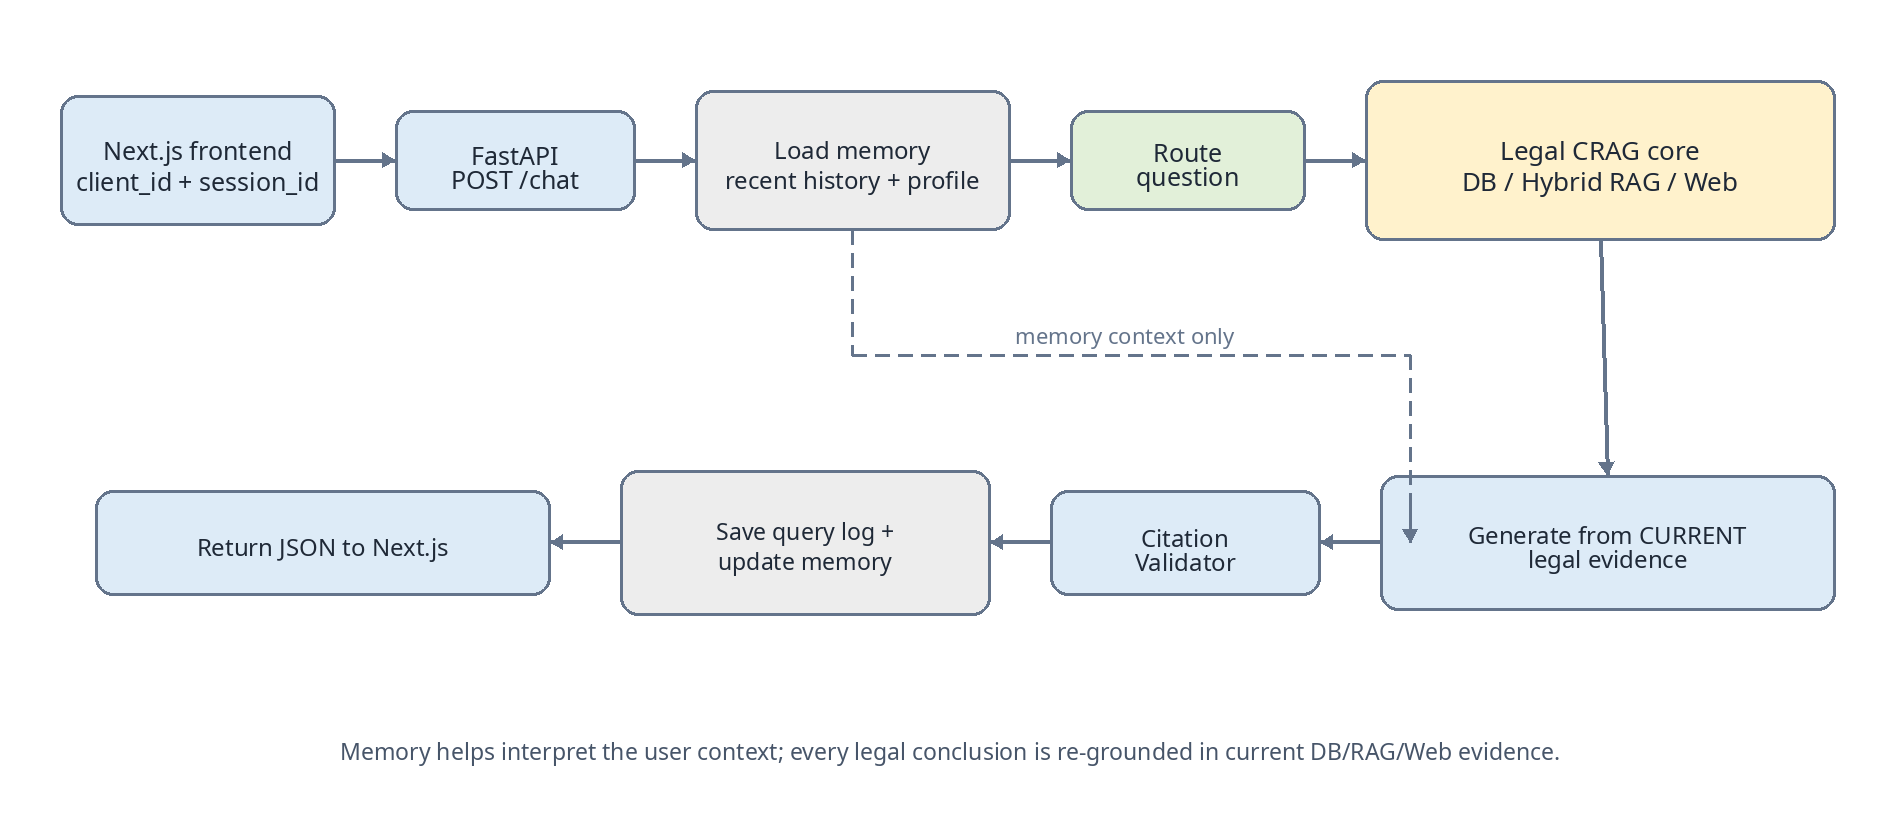
\includegraphics[width=\textwidth]{images/figure_3.png}
    \caption{Thứ tự thực hiện chuẩn mực: Ưu tiên dữ liệu, đo lường và lõi CRAG trước khi xây dựng giao diện người dùng.}
    \label{fig:implementation_flow}
\end{figure}

\begin{table}[htbp]
\centering
\caption{Kế hoạch thực hiện dự án theo 17 giai đoạn chuẩn hóa}
\label{tab:17_phases}
\renewcommand{\arraystretch}{1.2}
\rowcolors{2}{tablerowalt}{white}
\begin{tabularx}{\textwidth}{C{1.2cm} L{5.8cm} Y}
\toprule
\rowcolor{tableheader}\color{white}\textbf{Giai đoạn} & \color{white}\textbf{Công việc chi tiết} & \color{white}\textbf{Sản phẩm đầu ra (Deliverables)} \\
\midrule
1 & Xác định phạm vi và chính sách nguồn dữ liệu & Danh mục 50--100 văn bản pháp lý chính thống. \\
2 & Thu thập và bóc tách văn bản thô & Thư mục \texttt{data/raw} và \texttt{data/processed}. \\
3 & Chuẩn hóa siêu dữ liệu và quan hệ sửa đổi & Cơ sở dữ liệu SQLite \texttt{app.db} với các bảng quan hệ. \\
4 & Xây dựng tập hiệu chuẩn và tập kiểm thử & Tệp \texttt{calibration\_set.json} và \texttt{test\_set.json}. \\
5 & Cài đặt hệ thống truy hồi vector ngữ nghĩa & Kho vector ChromaDB với mô hình nhúng BGE-M3. \\
6 & Tích hợp BM25, thuật toán RRF và Reranker & Module truy hồi lai hoàn chỉnh. \\
7 & Cài đặt bộ đánh giá truy hồi và chọn ngưỡng & Cặp giá trị tối ưu $(T_{low}, T_{high})$ trên tập hiệu chuẩn. \\
8 & Hiện thực cơ chế tinh lọc tri thức & Nhánh Correct bóc tách các dải quy định cụ thể. \\
9 & Viết lại truy vấn và tìm kiếm web chính thống & Nhánh Incorrect với bộ lọc tên miền cho phép. \\
10 & Thuật toán hợp nhất và khử trùng lặp bằng chứng & Nhánh Ambiguous tích hợp đa nguồn. \\
11 & Xây dựng bộ kiểm định trích dẫn xác định & Module kiểm tra tính xác thực và hiệu lực trích dẫn. \\
12 & Hoàn thiện lõi tác tử LangGraph ReAct & Đồ thị StateGraph điều phối toàn bộ chu trình CRAG. \\
13 & Đo lường các hệ thống đối chứng và chỉ số RAGAS & Bảng số liệu thực nghiệm và vết thực thi LangFuse. \\
14 & Phát triển cổng API FastAPI và giao diện Next.js & Giao diện tra cứu và bảng trích dẫn căn cứ pháp luật. \\
15 & Tích hợp lịch sử hội thoại và hồ sơ ngữ nghĩa & Module lưu trữ phiên hội thoại SQLite. \\
16 & Đánh giá thử nghiệm A/B bộ nhớ & Báo cáo an toàn cách ly đạt Cross-client = 0. \\
17 & Hoàn thiện báo cáo kỹ thuật và trình diễn & Bản báo cáo LaTeX và mã nguồn nghiệm thu. \\
\bottomrule
\end{tabularx}
\end{table}

\section{Đề cương chi tiết 8 chương của báo cáo kỹ thuật}

Báo cáo kỹ thuật tốt nghiệp hoặc đồ án môn học chuẩn Thạc sĩ được phân bổ theo 8 chương:
\begin{enumerate}
    \item \textbf{Chương 1 -- Giới thiệu:} Bối cảnh ảo giác do truy hồi sai trong lĩnh vực pháp lý; bài toán trợ lý tuân thủ pháp lý doanh nghiệp; mục tiêu và năm câu hỏi nghiên cứu; phạm vi; các đóng góp chính của đề tài.
    \item \textbf{Chương 2 -- Cơ sở lý thuyết:} Tổng quan mô hình ngôn ngữ lớn nội bộ; tác tử AI có trạng thái; kiến trúc RAG cổ điển; truy hồi ngữ nghĩa với BGE-M3; BM25 và truy hồi lai; mô hình xếp hạng lại Cross-Encoder; LangGraph; nguyên lý Corrective RAG; khung đánh giá RAGAS; lý thuyết về bộ nhớ trong tác tử.
    \item \textbf{Chương 3 -- Phân tích và thiết kế hệ thống:} Đặc tả yêu cầu người dùng; kiến trúc ba tầng; luồng hoạt động chi tiết của LangGraph ReAct; thiết kế cơ sở dữ liệu pháp lý và quan hệ sửa đổi; mô hình trạng thái tác tử; chính sách kiểm soát nguồn web; thiết kế hệ thống kiểm định trích dẫn.
    \item \textbf{Chương 4 -- Chuẩn bị dữ liệu và tri thức:} Thu thập dữ liệu từ các cổng công quyền; kỹ thuật phân đoạn pháp lý; chuẩn hóa siêu dữ liệu; mô hình hóa lịch sử văn bản; lập chỉ mục vector Chroma và chỉ mục từ khóa BM25.
    \item \textbf{Chương 5 -- Xây dựng hệ thống tác tử:} Hiện thực truy hồi lai, RRF và Cross-Encoder; xây dựng bộ đánh giá với hai ngưỡng; chi tiết hóa ba nhánh CRAG; bộ sinh có cấu trúc JSON; kiểm định trích dẫn; kết nối FastAPI và giao diện Next.js; giám sát qua LangFuse.
    \item \textbf{Chương 6 -- Thiết kế thực nghiệm:} Phân tách tập hiệu chuẩn và tập kiểm thử độc lập; thiết kế các hệ thống đối chứng $S_0$--$S_4$; các phép thử phân tách thành phần; hệ thống các chỉ số truy hồi, điều hướng, chất lượng sinh và chuẩn mực pháp lý; quy trình quét lưới chọn ngưỡng.
    \item \textbf{Chương 7 -- Kết quả thực nghiệm và thảo luận:} Đánh giá chất lượng truy hồi; ma trận nhầm lẫn của bộ đánh giá; hiệu quả xử lý ba nhánh CRAG; phân tích các lượt gọi tìm kiếm ngoài; độ chính xác trích dẫn; phân tích các trường hợp thất bại thực tế.
    \item \textbf{Chương 8 -- Kết luận và hướng phát triển:} Đánh giá mức độ hoàn thành so với mục tiêu ban đầu; các hạn chế tồn đọng; đề xuất hướng mở rộng (đồ thị tri thức pháp lý, can thiệp của con người trong vòng lặp, tự động hóa cập nhật phiên bản).
\end{enumerate}

% !TEX root = ../main.tex
\chapter{Phụ lục và tài liệu tham khảo}

\section{Phụ lục A: Danh mục tệp mã nguồn chuẩn hóa}

\begin{table}[htbp]
\centering
\caption{Danh mục các module mã nguồn trong hệ thống -- Phần 1: Tác tử, công cụ và truy hồi}
\label{tab:source_files_part1}
\renewcommand{\arraystretch}{1.25}
\rowcolors{2}{tablerowalt}{white}
\begin{tabularx}{\textwidth}{L{4.8cm} Y}
\toprule
\rowcolor{tableheader}\color{white}\textbf{Tên tệp / Thư mục} & \color{white}\textbf{Mục đích và chức năng thực thi} \\
\midrule
\texttt{config.py} & Cấu hình tham số mô hình, Top-K, cặp ngưỡng $(T_{low}, T_{high})$, danh sách cho phép và đường dẫn hệ thống. \\
\texttt{llm.py} & Khởi tạo mô hình ngôn ngữ lớn đa nhà cung cấp (Groq, OpenAI, Ollama) theo Factory Pattern và mô hình nhúng BGE-M3. \\
\texttt{agent/state.py} & Định nghĩa cấu trúc trạng thái \texttt{AgentState} dạng TypedDict với các kênh tích lũy. \\
\texttt{agent/graph.py} & Thiết lập đồ thị StateGraph và rẽ nhánh ReAct (\texttt{agent}, \texttt{tools}, \texttt{cite\_validate}). \\
\texttt{agent/nodes.py} & Cài đặt các hàm xử lý logic tại từng nút của đồ thị LangGraph. \\
\texttt{agent/runtime.py} & Điểm vào duy nhất điều phối một lượt hội thoại: \texttt{prepare\_turn}, \texttt{persist\_turn}, \texttt{invoke\_crag}. \\
\texttt{agent/context.py} & Bộ quản lý ngữ cảnh lắp ghép lịch sử ngắn hạn (\texttt{messages}) và hồ sơ dài hạn (\texttt{memories}). \\
\texttt{tools/base.py} & Lớp cơ sở \texttt{BaseLegalTool} định nghĩa giao diện và lược đồ chuẩn cho công cụ tác tử. \\
\texttt{tools/registry.py} & Quản lý đăng ký tập trung và phân phối các lệnh gọi công cụ từ lõi tác tử. \\
\texttt{tools/crag\_search.py} & Công cụ tra cứu nội bộ: truy hồi lai, hợp nhất RRF, Cross-Encoder, bộ đánh giá ba nhánh và tinh lọc dải quy định. \\
\texttt{tools/web\_search.py} & Công cụ tìm kiếm web chính thống: viết lại truy vấn, lọc tên miền công quyền, làm sạch mã nguồn HTML. \\
\texttt{retrieval/dense.py} & Truy hồi vector ngữ nghĩa với ChromaDB và mô hình nhúng BGE-M3. \\
\texttt{retrieval/bm25.py} & Truy hồi từ khóa chính xác với thuật toán BM25Okapi. \\
\texttt{retrieval/fusion.py} & Hợp nhất danh sách xếp hạng ứng viên bằng giải thuật Reciprocal Rank Fusion ($k=60$). \\
\texttt{retrieval/reranker.py} & Mô hình Cross-Encoder BGE-Reranker-v2-m3 tái xếp hạng và tính điểm liên quan chuẩn hóa hàm Sigmoid. \\
\texttt{retrieval/refine.py} & Tinh chế tri thức: bóc tách đoạn trích thành các dải quy định pháp lý và lọc ngưỡng tối thiểu 0.40. \\
\bottomrule
\end{tabularx}
\end{table}

\begin{table}[htbp]
\centering
\caption{Danh mục các module mã nguồn trong hệ thống -- Phần 2: Nghiệp vụ, nạp tri thức, bộ nhớ và giao diện}
\label{tab:source_files_part2}
\renewcommand{\arraystretch}{1.25}
\rowcolors{2}{tablerowalt}{white}
\begin{tabularx}{\textwidth}{L{4.8cm} Y}
\toprule
\rowcolor{tableheader}\color{white}\textbf{Tên tệp / Thư mục} & \color{white}\textbf{Mục đích và chức năng thực thi} \\
\midrule
\texttt{legal/cleaner.py} & Làm sạch chuyên sâu: loại bỏ biểu mẫu chấm, số trang, khối nơi nhận, chuẩn hóa bảng mã Unicode NFC. \\
\texttt{legal/parser.py} & Phân tách cấu trúc văn bản pháp quy theo thứ bậc: Phần $\to$ Chương $\to$ Điều $\to$ Khoản $\to$ Điểm. \\
\texttt{legal/citations.py} & Bộ kiểm định trích dẫn xác định: kiểm tra sự tồn tại của \texttt{source\_id} và tính hiệu lực theo thời gian. \\
\texttt{legal/temporal.py} & Mô hình hóa lịch sử văn bản và phân giải quan hệ sửa đổi, bổ sung, thay thế. \\
\texttt{ingestion/worker.py} & Tiến trình xử lý ngầm đa luồng thực thi quy trình nạp tài liệu tự động. \\
\texttt{ingestion/chunks.py} & Thuật toán Legal-aware Chunking bảo toàn nguyên vẹn Điều luật và làm giàu tiêu đề ngữ cảnh. \\
\texttt{ingestion/indexer.py} & Quản trị đồng bộ hóa chỉ mục vector ChromaDB và chỉ mục từ khóa BM25. \\
\texttt{memory/store.py} & Quản lý cơ sở dữ liệu SQLite: phiên làm việc, nhật ký tin nhắn và thuộc tính người dùng. \\
\texttt{memory/extractor.py} & Trích xuất thuộc tính doanh nghiệp bền vững dựa trên danh mục cho phép \texttt{ALLOWED\_MEMORY\_KEYS}. \\
\texttt{eval/run\_eval.py} & Kịch bản tự động hóa đo lường kiểm chuẩn trên tập hiệu chuẩn và tập kiểm thử độc lập. \\
\texttt{eval/metrics.py} & Cài đặt công thức tính toán chỉ số truy hồi, điều hướng, RAGAS và kiểm định trích dẫn. \\
\texttt{api/main.py} & Hạ tầng FastAPI cung cấp các điểm cuối RESTful và SSE streaming thời gian thực. \\
\texttt{frontend/} & Ứng dụng Next.js 14 và TypeScript cung cấp giao diện tương tác người dùng và trang quản trị. \\
\texttt{schema.sql} & Bản đặc tả DDL của 8 bảng quan hệ chuẩn hóa trong cơ sở dữ liệu SQLite \texttt{app.db}. \\
\bottomrule
\end{tabularx}
\end{table}

\section{Phụ lục B: Phân công công việc nhóm phát triển}

\begin{table}[htbp]
\centering
\caption{Mô hình phân công trách nhiệm trong nhóm thực hiện đề tài}
\label{tab:team_roles}
\renewcommand{\arraystretch}{1.25}
\rowcolors{2}{tablerowalt}{white}
\begin{tabularx}{\textwidth}{L{4.2cm} Y}
\toprule
\rowcolor{tableheader}\color{white}\textbf{Vai trò thành viên} & \color{white}\textbf{Nội dung công việc phụ trách chính} \\
\midrule
\textbf{Thành viên 1 -- Kỹ sư Dữ liệu} & Thu thập văn bản từ cổng thông tin nhà nước; lập trình parser bóc tách điều khoản; chuẩn hóa siêu dữ liệu và quan hệ sửa đổi; thiết kế và quản trị SQLite \texttt{app.db}; xây dựng đường ống nạp dữ liệu và tích hợp Vision LLM OCR. \\
\textbf{Thành viên 2 -- Chuyên viên Truy hồi} & Triển khai kho vector ChromaDB với BGE-M3; cài đặt thuật toán BM25Okapi; lập trình giải thuật hợp nhất RRF; tích hợp mô hình xếp hạng lại Cross-Encoder BGE-Reranker-v2-m3; đo lường các chỉ số Recall@K và MRR. \\
\textbf{Thành viên 3 -- Lõi Tác tử \& CRAG} & Hiện thực bộ đánh giá truy hồi; cài đặt ba nhánh Correct, Ambiguous, Incorrect; xây dựng cơ chế tinh lọc tri thức và tìm kiếm web có kiểm soát; lập trình đồ thị tác tử LangGraph ReAct. \\
\textbf{Thành viên 4 -- Kiểm chuẩn \& Đảm bảo} & Xây dựng căn cứ sự thật cho tập hiệu chuẩn và tập kiểm thử độc lập; thực hiện quét lưới chọn cặp ngưỡng; đo lường các chỉ số RAGAS và Fallback; cấu hình giám sát LangFuse và phân tích các ca thất bại. \\
\textbf{Thành viên 5 -- Giao diện \& Bộ nhớ} & Phát triển ứng dụng Next.js 14 và API FastAPI hỗ trợ luồng SSE streaming; xây dựng hệ thống bộ nhớ phiên và hồ sơ ngữ nghĩa; thực hiện kiểm thử an toàn cách ly dữ liệu đa người dùng. \\
\bottomrule
\end{tabularx}
\end{table}

\section{Phụ lục C: Tiêu chí tự kiểm tra chất lượng trước khi nghiệm thu}

\begin{calloutbox}{Bảng kiểm tra điều kiện nghiệm thu hệ thống}
\begin{itemize}
    \item Có ít nhất một ca kiểm thử \textbf{Correct} trả lời chính xác và dẫn nguồn trích dẫn hợp lệ.
    \item Có ít nhất một ca kiểm thử \textbf{Incorrect} kích hoạt thành công tìm kiếm web có kiểm soát.
    \item Có ít nhất một ca kiểm thử \textbf{Ambiguous} hợp nhất thành công tri thức nội bộ và mở rộng.
    \item Có ít nhất một truy vấn siêu dữ liệu hoặc định vị điều khoản trực tiếp từ cơ sở dữ liệu quan hệ SQLite.
    \item Vết thực thi (\textit{execution trace}) thể hiện rõ điểm số đánh giá và nhánh rẽ được lựa chọn.
    \item Bảng thực nghiệm so sánh đầy đủ giữa Traditional RAG, RAG + Always Web và Full CRAG.
    \item Tập hiệu chuẩn được phân tách độc lập hoàn toàn khỏi tập kiểm thử độc lập.
    \item Bộ kiểm định trích dẫn chứng minh được khả năng phát hiện và chặn câu trả lời trích dẫn sai.
    \item Có phân tích ca thất bại thực tế kèm chẩn đoán nguyên nhân gốc rễ.
    \item Tuyệt đối không sử dụng dữ liệu bộ nhớ làm nguồn căn cứ pháp lý.
    \item Đạt chỉ số an toàn tuyệt đối: Cross-client Contamination = 0.
\end{itemize}
\end{calloutbox}

\section*{Tài liệu tham khảo}
\addcontentsline{toc}{section}{Tài liệu tham khảo}

\begin{enumerate}[label={[\arabic*]}]
    \item Yan, S.-Q., Gu, J.-C., Zhu, Y., \& Ling, Z.-H. (2024). \textit{Corrective Retrieval Augmented Generation}. arXiv preprint arXiv:2401.15884v3.
    \item Lewis, P., Perez, E., Piktus, A., Petroni, F., Karpukhin, V., Goyal, N., \dots \& Kiela, D. (2020). \textit{Retrieval-Augmented Generation for Knowledge-Intensive NLP Tasks}. Advances in Neural Information Processing Systems, 33, 9459--9474.
    \item Asai, A., Sewon, M., Jiang, Z., Chen, X., Zettlemoyer, L., \& Hajishirzi, H. (2024). \textit{Self-RAG: Learning to Retrieve, Generate, and Critique through Self-Reflection}. International Conference on Learning Representations (ICLR).
    \item Es, S., James, J., Espinosa-Anke, L., \& Schockaert, S. (2023). \textit{RAGAS: Automated Evaluation of Retrieval Augmented Generation}. arXiv preprint arXiv:2309.15217.
    \item Cormack, G. V., Clarke, C. L., \& Buettcher, S. (2009). \textit{Reciprocal Rank Fusion Outperforms Condorcet and Individual Rank Learning Methods}. Proceedings of the 32nd International ACM SIGIR Conference.
    \item Yao, S., Zhao, J., Yu, D., Du, N., Shafran, I., Narasimhan, K., \& Cao, Y. (2023). \textit{ReAct: Synergizing Reasoning and Acting in Language Models}. International Conference on Learning Representations (ICLR).
    \item Quốc hội Nước Cộng hòa Xã hội Chủ nghĩa Việt Nam. (2020). \textit{Luật Doanh nghiệp số 59/2020/QH14}.
    \item Quốc hội Nước Cộng hòa Xã hội Chủ nghĩa Việt Nam. (2019). \textit{Bộ luật Lao động số 45/2019/QH14}.
    \item BAAI (Beijing Academy of Artificial Intelligence). (2024). \textit{BGE-M3 and BGE-Reranker-v2-m3 Models Documentation}. Hugging Face Model Hub.
    \item LangChain Inc. (2024). \textit{LangGraph: Multi-Agent and Stateful Graph Orchestration Reference}. https://langchain-ai.github.io/langgraph/.
    \item Groq Inc. (2024). \textit{Groq LPU Inference Engine Documentation \& API Reference}. https://groq.com.
    \item OpenRouter. (2024). \textit{Unified LLM Interface \& Routing Documentation}. https://openrouter.ai.
\end{enumerate}

\label{LastPage}
\end{document}
